\documentclass{book}

\usepackage{iftex}

\ifxetex
\usepackage{fontspec}
\usepackage{ebgaramond}
\else
\usepackage{alternative4ht}
\altusepackage{fontspec}
\fi
%\newfontfamily\pIqaD{pIqaD-qolqoS.ttf}
\newfontface  \pIqaD{pIqaD-qolqoS.ttf}
%\setmainfont[Ligatures=TeX]{ebgaramond}

%\usepackage[utf8]{inputenc}
%\usepackage[T1]{fontenc}
\usepackage[finnish]{babel}
\usepackage[a5paper]{geometry}
\usepackage{dcolumn}
\usepackage{multirow}
\usepackage{amssymb}
\usepackage[xindy]{imakeidx}
\usepackage{longtable}
\usepackage{enumitem}
\usepackage{hyperref}
\usepackage{tikz}

\usetikzlibrary{shapes.geometric,arrows,arrows.meta}
\usetikzlibrary{shapes.multipart}

\makeindex[title=Käsitteiden hakemisto]
\makeindex[name=sanat,title=Klingonin sanojen hakemisto]

\title{{\pIqaD   }\\Klingonin kielioppi}
\author{Iikka Hauhio}

\setlength{\parindent}{0cm}
\setlength{\parskip}{1em}
\setlist[itemize]{parsep=0pt}
\setlist[enumerate]{parsep=0pt}
\newcolumntype{B}[0]{>{\bfseries}}
\newcolumntype{I}[0]{>{\itshape}}
\newcolumntype{T}[0]{>{\pIqaD}}

\begin{document}

\frontmatter

\maketitle

\newpage
\vspace*{\fill}
1. painos

© 2021 Iikka Hauhio

%\textbf{Osittainen kopiointikielto} \\
%Tämän teoksen kopioiminen on tekijänoikeuslain (404/61, muut. 849/18) mukaisesti kielletty lukuunottamatta Suomen valtion ja Kopiosto r.y.:n tekemässä sopimuksessa tarkemmin määriteltyä osittaista kopiointia opetustarkoituksiin.

\textbf{Kopiointi sallittu} \\
Tämän teoksen kopiointi on sallittu Creative Commons Nimeä 4.0 Kansainvälinen -lisenssin ehdoilla.
Kopiointi, muokkaaminen ja jakaminen on sallittu, mutta alkuperäisen tekijän nimi on ilmoitettava.

http://creativecommons.org/licenses/by/4.0/

\chapter{Alkusanat}

Tämä on yritys soveltaa olemassaolevaa kielitieteen käsitteistöä klingoniin.
Kielen ominaisuudet on kuvattu lyhyesti ja jokaisesta kuvatusta ilmiöstä on joukko esimerkkilauseita.
Tyylillisesti kirja yrittää mukailla lukion oppilaille suunnattuja kielioppeja.

Koska kirja on tarkoitettu myös vasta-alkajille, klingoni on kirjoitettu romanisoiduilla aakkosilla klingonin oman pIqaD-aakkoston sijaan.
Se ei ole oppikirja, vaan sitä on tarkoitus käyttää viiteteoksena muun kurssimateriaalin tukena.

Koska vasta opettelen klingonia kirjoittaessani tätä, tekstissä saattaa olla virheitä.

\begin{quote}
    Iikka Hauhio \\
    \textit{Helsingissä lokakuussa 2020}
\end{quote}

\chapter{'et mu'}

tlhIngan Hol vIrIchtaHvIS HolQeD mu' tu'lu'bogh vIlo'meH, paqvam vIqonta'.
nom pab vIDel 'ej ghantoH mu'tlheghmey ghaj paq Hoch 'ay'.
patlh cha'DIch DuSaQ jen pab paqmey rur paqvam 'e' vInID.

ghojwI' chu'vaD paqvam vIqonta'mo', tlhIngan Hol mu'meyvaD roma'ngan ngutlhmey vIlo' 'ej pIqaD vIlo'be'.
ghojmeH paq 'oHbe' paqvam'e'. pab ngaS neH. latlh DuSaQ paqmey lulaDlu'taHvIS, paqvam lo'lu'.

paqvam vIqontaHvIS tlhIngan Hol vIghojtaHmo' neH, chaq Qagh tu'lu'.
vay' bolu'chugh, HISovmoH.

\begin{quote}
    'Iyqa HawHI'o \\
    \textit{HelsIngqIDaq, tera' jar wa'maH, tera' DIS 2020}
\end{quote}

\tableofcontents

\mainmatter

\chapter{Johdanto}

Klingon on yhdysvaltalaisen kielitietelijän, tohtori Marc Okrandin kehittämä fiktiivinen keinotekoinen kieli. Sen alkuperäinen tarkoitus oli toimia Star Trek -universumissa elävien klingonien kansalliskielenä. Tähän mennessä klingonin kieltä on käytetty kuudessa Star Trek -elokuvassa, kahdessa televisiosarjassa\footnote{Star Trek: Enterprise ja Star Trek: Discovery. Muissa televisiosarjoissa ei puhuta oikeaa klingonin kieltä.} ja useissa Okrandin kirjoittamissa kirjoissa. Tämän lisäksi kielellä on oma harrastajayhteisönsä, joka on tuottanut lukuisia klingoninkielisiä teoksia.

Kielenä klingon ei ole sukua millekään maapallon kielelle, ja monet sen ominaisuudet on tarkoituksella valittu siten, että ne ovat mahdollisimman harvinaisia ihmiskielissä. Klingonin sanoja ei ole suoraan lainattu mistään muusta kielestä hyvin pientä määrää lainasanoja lukuunottamatta. Monet sanat perustuvat sen sijaan sanaleikkeihin ja vitseihin.

Marc Okrandia pidetään klingonin ylimpänä auktoriteettina ja hänen kirjoittamaansa klingonia pidetään määritelmällisesti hyvänä. Klingoninkielinen teksti voidaankin jakaa Okrandin kirjoittamaan \textit{kanoniseen klingoniin} ja harrastelijoiden tuottamaan \textit{epäkanoniseen klingoniin}. Tärkeimpiä kanonisia teoksia ovat kielioppia ja sanastoa käsittelevät \textit{The Klingon Dictionary}, \textit{Klingon for Galactic Traveler}, mietelausekokoelma \textit{The Klingon Way} ja runoeepos \textit{paq'batlh}. Näiden lisäksi kanonisina lähteinä pidetään Okrandin haastatteluja eri lehdissä ja medioissa sekä sekalaisia muita hänen tekemiään klingontekstejä.

Valitettavasti kanoniset lähteet ovat monesti epäselviä tai ristiriidassa keskenään. Eräs suuri epäselvyysongelma liittyy Okrandin klingon-englanti-sanakirjaan, johon ei ole merkitty verbien transitiivisuuksia. Klingonissa, kuten suomessa ja toisin kuin englannissa, verbit ovat yleensä joko transitiivisia tai intransitiivisia, mutta eivät molempia: klingonissa on esimerkiksi erikseen verbit \textbf{pum} \textit{pudota} ja \textbf{pummoH} \textit{pudottaa}. Kuitenkaan monien sanojen englanninkielisistä käännöksistä ei voi tietää kumpi merkitys on kyseessä, sillä englannissa sama sana on usein sekä intransitiivinen että transitiivinen. Esimerkiksi sana \textbf{tet} on käännetty Okrandin sanakirjassa vain \textit{melt} (\textit{sulaa} tai \textit{sulattaa}). Monet uskoivat sanan tarkoittavan \textit{sulaa}, olisihan silloin mahdollista yhä sanoa \textbf{*tetmoH} \textit{sulattaa}, mutta itse asiassa myöhemmin Okrand on käyttänyt sanaa merkityksessä \textit{sulattaa}. Ei ole tiedossa miten klingoniksi voi sanoa intransitiivisen merkityksen \textit{sulaa}.

Ristiriitaisuudet ovat toinen suuri ongelma. Ne saattavat johtua siitä, että Okrand on unohtanut aiemmin kehittämiään sääntöjä, tai vain kirjoitus- tai ajatusvirheistä. Eräs ristiriita liittyy lokatiivisijamuodon (\textbf{-Daq}) merkitykseen: aiemmin Okrand on käyttänyt liikkumisverbien \textbf{ghoS}, \textbf{jaH}, ym. yhteydessä sitä sekä merkityksessä \textit{jonnekin} että \textit{jossakin}. Kuitenkin myöhemmin hän on väittänyt sen merkitsevän vain \textit{jossakin}. Klingoninharrastajat eivät tiedä miten suhtautua tähän ja toistavat joskus vanhoja sääntöjä ja joskus uusia sääntöjä.

Tässä kirjassa kiistellyt säännöt on ilmaistu sanoilla ''pidetään huonona kielenkäyttönä''. Nämä sanat tarkoittavat, että sääntöä saatetaan rikkoa kaanonissa tai että se on uusi ja on ristiriidassa aiempien sääntöjen kanssa.

Tämä kirja on oma tulkintansa klingonin kieliopista eikä käytä samaa käsitteistöä tai rakennetta kuin Okrandin virallinen kielioppiteos \textit{The Klingon Dictionary}. Eroja on käsitelty tarkemmin liitteessä~\ref{apx:perinne}.

\chapter{Substantiivit}

\section{Substantiivin suku}
\index{suku}

Klingonin substantiivit jaetaan kolmeen sukuun:

\begin{enumerate}
\item Henkilöt
\item Ruumiinosat
\item Muut sanat
\end{enumerate}

\subsection{Henkilöt}

Ihmiset, klingonit, ihmisiin rinnastettavat tekoälyt, muut älykkäät kieltä käyttävät olennot\\*[1em]
\begin{tabular}{Bl Il}
nuv & henkilö \\
puq & lapsi \\
Human & ihminen \\
tera'ngan & maan asukas \\
tlhIngan & klingoni \\
SuvwI' & soturi \\
ghojmoHwI' & opettaja \\
ghu & vauva \\
\end{tabular}

\subsection{Ruumiinosat}

Raajat, elimet, muut ruumiinosat (ei ruumis kokonaisuutena)\\*[1em]
\begin{tabular}{Bl Il}
ghIch & nenä \\
ghop & käsi \\
tIq & sydän \\
DIr & iho \\
\end{tabular}

Sanat kuuluvat tähän sukuun yleensä vaikka ne olisivat vertauskuvallisia tai alkuperäinen merkitys on muuten etääntynyt.\\*[1em]
\begin{tabular}{Bl Il}
    Ho'Du' & sankarit \\
\end{tabular}

\subsection{Muut sanat}

Eläimet, ei-älykkäät elämänmuodot, esineet, asiat, käsitteet\\*[1em]
\begin{tabular}{Bl Il}
Duj & alus \\
porgh & vartalo \\
yab & mieli \\
qoq & robotti \\
qaghwI' & '-merkki \\
\end{tabular}

\section{Liitteiden järjestys}

Klingonissa substantiiviliitteiden on aina oltava seuraavalla tavalla järjestyksessä:\\*[1em]
\begin{tabular}{l Bl}
juuri & Duj \\
johdin & -Hom \\
täsmennysliite & -qoq \\
monikon tunnnus & -mey \\
omistusliite tai demonstratiiviliite & -lIj \\
sijapääte & -mo' \\
\end{tabular}

\textbf{DujHomqoqmeylIjmo'} \textit{Sinun niin kutsuttujen pikku alustesi vuoksi}

\section{Johdinliitteet}
\index[sanat]{-'a'}
\index[sanat]{-Hom}
\index[sanat]{-oy}

\begin{tabular}{l Bl | Bl Il}
    augmentatiivi & -'a' & veS'a' & suuri sota \\
    diminutiivi 1 & -Hom & vengHom & kylä (pieni kaupunki) \\
    diminutiivi 2 & -oy & vavoy & isi \\
\end{tabular}

\textbf{-Hom}-liitteellä on halveksiva sävy, ja \textbf{-oy}-liitteellä on hellittelevä sävy.

\section{Täsmennysliitteet}
\index{täsmennysliitteet}
\index[sanat]{-qoq}
\index[sanat]{-Hey}
\index[sanat]{-na'}

Täsmennysliiteellä voi ilmaista, kuinka sopiva käytetty sana puhujan mielestä on.\\*[1em]
\begin{tabular}{Bl l}
    -qoq & ''niin kutsuttu'' \\
    -Hey & ''ilmeisesti'': puhuja ei ole varma onko käytetty sana oikea \\
    -na' & ''varmasti'': puhuja on varma käyttämästään sanasta \\
\end{tabular}

Esimerkiksi:\\*[1em]
\begin{tabular}{l l}
    luj SuvwI'\textbf{qoq}. & Niin kutsuttu soturi hävisi. \\
    ghojwI'\textbf{Hey} 'oH puq'e'. & Lapsi on ilmeisesti oppilas. \\
    Duj\textbf{na'} vIleghpu'. & Näin varmasti aluksen. \\
\end{tabular}

\section{Monikko}
\index{monikko}
\index[sanat]{-pu'}
\index[sanat]{-Du'}
\index[sanat]{-mey}

Monikon tunnus riippuu suvusta.
Lisäksi joillakin ainesanoilla ei ole monikkomuotoa (kuten \textbf{'Iw} \textit{veri})
ja joillakin epäsäännöllisillä sanoilla käytetään monikkomuodon sijasta erityistä kieliopillisesti yksiköllistä monikkosanaa.\\*[1em]
\begin{tabular}{l Bl | Bl Il l}
henkilöt & -pu' & puqpu' & lapset & \\
ruumiinosat & -Du' & tIqDu' & sydämet & \\
muut & -mey & qoqmey & robotit & \\
epäsäännölliset & & ngop & lautaset & (\textbf{jengva'} \textit{lautanen}) \\
\end{tabular}

Jos \textbf{-mey}-liitettä käyttää henkilöiden tai epäsäännöllisten sanojen kanssa, sen merkitys on \textit{siellä täällä}:\\*[1em]
\begin{tabular}{l l}
    \textbf{puqmey} vIlegh. & Näin lapsia siellä täällä. \\
    qatlh \textbf{jengva'mey} tu'lu'? & Miksi lautasia on siellä täällä? \\
\end{tabular}

\section{Omistusliitteet}
\index{omistusliite}
\index[sanat]{-wI'}
\index[sanat]{-wIj}
\index[sanat]{-ma', -maj}
\index[sanat]{-lI'}
\index[sanat]{-lIj}
\index[sanat]{-ra', -raj}
\index[sanat]{-Daj}
\index[sanat]{-chaj}

Omistusliitteet riippuvat monikon tunnuksen tavoin omistettavan asian suvusta.\\*[1em]
\begin{tabular}{l Bc Bc}
& \multicolumn{2}{c}{omistettava asia} \\
& \multicolumn{1}{c}{henkilöt} & \multicolumn{1}{c}{muut} \\
minun & -wI' & -wIj \\
sinun & -lI' & -lIj \\
hänen/sen & \multicolumn{2}{Bc}{-Daj} \\
meidän & -ma' & -maj \\
teidän & -ra' & -raj \\
heidän/niiden & \multicolumn{2}{Bc}{-chaj} \\
\end{tabular}

Esimerkiksi:\\*[1em]
\begin{tabular}{Bl Il}
tIqwIj & sydämeni \\
puqlI' & lapsesi \\
batlhmaj & kunniamme \\
juHDaj & (hänen) kotinsa \\
\end{tabular}

\section{Demonstratiiviliitteet}
\index{demonstratiiviliite}
\index[sanat]{-vam}
\index[sanat]{-vetlh}

Demonstratiiviliitteet osoittavat mistä tai kenestä on kysymys.
Klingon kielessä on kaksi demonstratiiviliitettä:\\*[1em]
\begin{tabular}{Bl Il}
    -vam & tämä \\
    -vetlh & tuo \\
\end{tabular}

Demonstratiiviliitettä ja omistusliitettä ei voi käyttää yhtä aikaa.\\*[1em]
\begin{tabular}{Bl Il}
    paqvam & tämä kirja \\
    nuvpu'vam & nämä henkilöt \\
    Humanvetlh & tuo ihminen \\
    yabmeyvetlh & nuo mielet \\
\end{tabular}

\section{Sijamuodot}
\index{sijamuodot}

Klingonin kielessä on kuusi sijamuotoa.\\*[1em]
\begin{tabular}{l Bl | Bl Il}
nominatiivi & - & Duj & alus \\
lokatiivi & -Daq & DujDaq & aluksessa, alukseen \\
elatiivi & -vo' & Dujvo' & aluksesta \\
datiivi & -vaD & DujvaD & alukselle \\
kausatiivi & -mo' & Dujmo' & aluksen vuoksi \\
aiheellistin & -'e' & Duj'e' & alus \\
\end{tabular}

\subsection{Nominatiivi}
\index{nominatiivi}

Nominatiivia käytetään

1. ilmaisemaan lauseen subjektia ja objektia
\index{subjekti}
\index{objekti}\\*[1em]
\begin{tabular}{l l}
    qet \textbf{puqpu'}. & Lapset juoksevat. \\
    \textbf{Soj} vISop. & Syön ruokaa. \\
\end{tabular}

2. ilmaisemaan omistamista\\*[1em]
\begin{tabular}{l l}
    \textbf{be'} paq vIlaD. & Luen naisen kirjaa. \\
    tIn \textbf{ghojmoHwI'} ghIch. & Opettajan nenä on suuri. \\
\end{tabular}

3. ilmaisemaan kansalaisuutta\\*[1em]
\begin{tabular}{l l}
    Dun \textbf{tlhIngan} wo'. & Klingon-valtakunta on suuremmoinen. \\
\end{tabular}

4. sanaliitoissa\\*[1em]
\begin{tabular}{l Il}
    \textbf{ropyaH} qach & sairaala \\
    \textbf{QIn} 'echletHom & postikortti \\
\end{tabular}

5. postposition edellä
\index{postpositio}\\*[1em]
\begin{tabular}{l l}
    \textbf{raS} bIngDaq 'oH tu'lu'. & Se on pöydän alla. \\
\end{tabular}

6. ilmaisemaan lauseen tapahtuma-aikaa\\*[1em]
\begin{tabular}{l l}
    \textbf{DaHjaj ram} vIQonglaHbe'. & En voi nukkua tänä yönä. \\
\end{tabular}

Jos ajanmääre kertoo tapahtuman keston, käytetään verbiä \textbf{qaStaHvIS} \textit{aikana}:\\*[1em]
\begin{tabular}{l l}
    \textbf{qaStaHvIS cha' rep} vIQongpu'. & Nukuin kaksi tuntia. \\
\end{tabular}

\subsection{Lokatiivi}
\index{lokatiivi}
\index[sanat]{-Daq}

Lokatiivia käytetään ilmaisemaan

1. sijaintia\\*[1em]
\begin{tabular}{l l}
    reH \textbf{juHwIjDaq} jISop. & Syön aina kotona. \\
\end{tabular}

2. määränpäätä\\*[1em]
\begin{tabular}{l l}
    \textbf{juHDaq} yIjaH! & Mene kotiin! \\
    'u' \textbf{HeHDaq} tlhIngan juHqo'vo'. & Klingonien kotimaailmasta \\
    & maailman laidalle. \\
\end{tabular}

Liikkumisverbien kuten \textbf{jaH} ja \textbf{ghoS} määränpää ilmaistaan suoralla objektilla, joka voidaan taivuttaa joko lokatiivissa tai nominatiivissa. Tällöin pidetään huonona kielenkäyttönä käyttää verbietuliitettä, jonka mukaan objektia ei ole (kuten \textbf{jI-}).\\*[1em]
\begin{tabular}{l l}
    \textbf{juHDaq / juH} vIjaH. & Menen kotiin. \\
    \textbf{juHDaq} jIjaH. & Menen kodissa / kotiin. \\
\end{tabular}

\subsection{Elatiivi}
\index{elatiivi}
\index[sanat]{-vo'}

Elatiivi ilmaisee lähtöpaikkaa.\\*[1em]
\begin{tabular}{l l}
    \textbf{yuQvamvo'} jIleng vIneH. & Haluan matkustaa pois tältä \\
    & planeetalta. \\
    \textbf{nachlIjvo'} mIv yItuQHa'moH! & Riisu kypärä päästäsi! \\
    \textbf{naDevvo'} bIQ'a' DaleghlaH. & Voit nähdä täältä meren. \\
\end{tabular}

\subsection{Datiivi}
\index{datiivi}
\index[sanat]{-vaD}

Datiivia käytetään

1. ilmaisemaan vastaanottajaa\\*[1em]
\begin{tabular}{l l}
    \textbf{SoHvaD} QIn ngeHpu' ghaH. & Hän lähetti sinulle viestin. \\
    \textbf{puqwI'vaD} Soj vIje'. & Ostan ruokaa lapselleni. \\
\end{tabular}

2. ilmaisemaan -moH-verbin kokijaa
\index[sanat]{-moH}\\*[1em]
\begin{tabular}{l l}
    \textbf{ghaHvaD} quHDaj qawmoH. & Se muistuttaa häntä perinnöstään. \\
\end{tabular}

3. pong-verbin kanssa\\*[1em]
\begin{tabular}{l l}
    \textbf{vavwI'vaD} ''vavoy'' vIpong. & Kutsun isääni ''vavoyksi''. \\
\end{tabular}

\subsection{Kausatiivi}
\index{kausatiivi}
\index[sanat]{-mo'}

Kausatiivia käytetään ilmaisemaan syytä\\*[1em]
\begin{tabular}{l l}
    \textbf{ropmo'} juHvo' jImejbe'. & En lähde kotoa sairauden takia. \\
\end{tabular}

\subsection{-'e'}
\index[sanat]{-'e'}

-'e'-sijamuotoa käytetään

1. ilmaisemaan predikatiivilauseen subjektia\\*[1em]
\begin{tabular}{l l}
    ghojmoHwI' ghaH \textbf{loDvetlh'e'}. & Tuo mies on opettaja. \\
\end{tabular}

2. lauseenvastikkeissa\\*[1em]
\begin{tabular}{l l}
    \textbf{Doch'e'} ghojmoHbogh ghaH Daqaw'a'? & Muistatko, mitä hän \\
    & opetti? \\
\end{tabular}

3. asettamaan aihe (seuraavat lauseet liittyvät aiheeseen)\\*[1em]
\begin{tabular}{l l}
    puj \textbf{vaj'e'}. tlhoy 'ugh yan. & Soturi on heikko, hänen miekkansa on \\
    & liian raskas. \\
\end{tabular}

4. painottamaan lauseen subjektia tai objektia\\*[1em]
\begin{tabular}{l l}
    'ut \textbf{Qu''e'}, 'utbe' latlh Doch. & Tehtävä on tärkeä, muut asiat \\
    & eivät. \\
\end{tabular}

5. vertailurakenteessa\\*[1em]
\begin{tabular}{l l}
    \textbf{QeD'e'}, HolQeD 'ut law', Hoch 'ut puS. & Kielitiede on tärkein tiede.
\end{tabular}

\chapter{Postpositiot}
\index{postpositio}

Klingonin postpositiot ilmaisevat paikkaa ja taipuvat paikallissijoissa (\textbf{-Daq}, \textbf{-vo'}).
\index[sanat]{-vo'}
\index[sanat]{-Daq}\\*[1em]
\begin{tabular}{Bl Il | Bl l}
    Dung & yläpuoli & qach DungDaq & rakennuksen yllä/ylle \\
    bIng & alapuoli & raS bIngDaq & pöydän alla/alle \\
    tlhop & etupuoli & Duj tlhopDaq & aluksen edessä/eteen \\
    'em & takapuoli & Dub 'emDaq & selän takana/taakse \\
    nIH & oikea puoli & loD nIHDaq & miehestä oikealla/e \\
    poS & vasen puoli & loD poSDaq & miehestä vasemmalla/e \\
    qoD & sisäpuoli & qach qoDDaq & rakennuksen sisällä/e \\
    Hur & ulkopuoli & Duj HurDaq & ulkona/ulos aluksesta \\
    joj & välitila & qachmey jojDaq & rakennusten välissä/väliin \\
    retlh & vieri & jup retlhDaq & ystävän vieressä/viereen \\
\end{tabular}
\index[sanat]{Dung}
\index[sanat]{bIng}
\index[sanat]{tlhop}
\index[sanat]{'em}
\index[sanat]{nIH}
\index[sanat]{poS}
\index[sanat]{qoD}
\index[sanat]{Hur}
\index[sanat]{joj}
\index[sanat]{retlh}

Postpositioihin ei lisätä omistusliitteitä, kun niitä käytetään persoonapronominien kanssa.\\*[1em]
\begin{tabular}{l l}
    \textbf{jIH bIngDaq} QemjIq tu'lu'. & Allani on kuoppa.
\end{tabular}

\chapter{Verbit}
\index{verbi}

\section{Adjektiivisuus}
\index{adjektiivi}

Klingonin verbit voidaan jakaa transitiivisiin ja intransitiivisiin.
Intransitiivisista verbeistä osa on adjektiivisia ja osa ei.
Adjektiiviset verbit vastaavat muiden kielten adjektiiveja.
\index{transitiivinen verbi}
\index{intransitiivinen verbi}\\*[1em]
\begin{tabular}{Bl Il | l l}
    ru' & olla väliaikainen & \textbf{ru'} roj. & Rauha on väliaikainen. \\
    tIn & olla suuri & \textbf{tIn} Dujvam. & Tämä alus on suuri. \\
    mach & olla pieni & \textbf{mach} ghunwI'. & Ohjelmoija on pieni. \\
    'ut & olla tärkeä & \textbf{'ut} Qu'. & Tehtävä on tärkeä. \\
\end{tabular}

Adjektiivinen verbiä voidaan käyttää attribuuttina pääsanansa jälkeen.
Tällöin verbillä voi olla vain päätteet \textbf{-Ha'}, \textbf{-be'} ja \textbf{-qu'}.\\*[1em]
\begin{tabular}{l l}
    roj \textbf{ru'} wIneH. & Haluamme väliaikaisen rauhan. \\
    Duj \textbf{tIn} vIghaj. & Minulla on iso alus. \\
    po' \textbf{ghunwI'} mach. & Pieni ohjelmoija on taitava. \\
    Qu' \textbf{'ut} yIqIlQo'! & Älä hylkää tärkeää tehtävää! \\
\end{tabular}

Substantiivin sijamuoto liitetään adjektiiviattribuuttiin, jos sellainen on.\\*[1em]
\begin{tabular}{l}
    ghunwI'pu' \textbf{machvaD} HolQeD vIghojmoH. \\
    Opetan kielitiedettä pienille ohjelmoijille. \\ 
\end{tabular}

Varsinaisia adjektiiviattribuutteja voi olla vain yksi. Verbillä voi kuitenkin olla useita partisiippimuotoisia (\textbf{-bogh}) adjektiiveja määreenä.\\*[1em]
\begin{tabular}{l}
    \textbf{chImbogh} 'ej \textbf{bIrbogh} 'antartIq \textbf{Hop} vIlegh vIneH. \\
    Haluan nähdä kaukaisen, aution ja kylmän Antarktiksen. \\
\end{tabular}
\index[sanat]{-bogh}

\section{-Ha'-johdin}
\index[sanat]{-Ha'}

\textbf{-Ha'}-johdin muuttaa verbin merkityksen usein vastakohtaiseksi.
Se liitetään aina verbin juureen.\\*[1em]
\begin{tabular}{Bl Il | Bl Il}
    par & inhota & parHa' & tykätä \\
    muS & vihata & musHa' & rakastaa \\
    quv & kunnioittaa & quvHa' & häpäistä \\
    nob & antaa & nobHa' & palauttaa \\
    ru' & olla väliaikainen & ru'Ha' & olla pysyvä \\
\end{tabular}

Joillakin verbeillä johtimen merkitys on \textit{tehdä väärin}.\\*[1em]
\begin{tabular}{Bl Il | Bl Il}
    jatlh & puhua & jatlhHa' & sanoa väärin \\
    yaj & ymmärtää & yajHa' & ymmärtää väärin \\
\end{tabular}

\section{Persoona}
\index{persoonamuodot}

Klingonin verbit kongruoivat sekä subjektin että objektin kanssa.
Persoonan tunnus on verbin etuliite.\\*[1em]
\begin{tabular}{Bc | Bc | Bc | Bc | Bc | Bc | Bc l}
    \multicolumn{7}{c}{Objekti} & Subjekti \\
    \multicolumn{1}{c}{jIH} & \multicolumn{1}{c}{maH} &\multicolumn{1}{c}{SoH} &\multicolumn{1}{c}{tlhIH} &\multicolumn{1}{c}{ghaH} &\multicolumn{1}{c}{chaH} &\multicolumn{1}{c}{-} & \\
    \multicolumn{1}{c}{} & \multicolumn{1}{c}{} &\multicolumn{1}{c}{} &\multicolumn{1}{c}{} &\multicolumn{1}{c}{'oH} &\multicolumn{1}{c}{bIH} &\multicolumn{1}{c}{} & \\
    - & - & qa- & Sa- & \multicolumn{2}{Bc |}{vI-} & jI- & jIH \\
    \cline{1-7}
    - & - & pI- & re- & wI- & DI- & ma- & maH \\
    \cline{1-7}
    cho- & ju- & - & - & \multicolumn{2}{Bc |}{Da-} & bI- & SoH \\
    \cline{1-7}
    tu- & che- & - & - & \multicolumn{2}{Bc |}{bo-} & Su- & tlhIH \\
    \cline{1-7}
    \multirow{2}{*}{mu-} & \multirow{2}{*}{nu-} & Du- & \multirow{2}{*}{lI-} &$\varnothing$- & \multicolumn{2}{Bc}{\multirow{2}{*}{$\varnothing$-}} & ghaH/'oH \\
    \cline{3-3}
    \cline{5-5}
    & & nI- & & lu- & \multicolumn{2}{c}{} & chaH/bIH \\
    \hline
    vI-lu' & wI-lu' & Da-lu' & bo-lu' & $\varnothing$-lu' & lu-lu' & - & (passiivi) \\
    \hline
    \multirow{2}{*}{HI-} & \multirow{2}{*}{gho-} & - & - & \multirow{2}{*}{yI-} & \multirow{2}{*}{tI-} & yI- & SoH (imp.)\\
    \cline{3-4}
    \cline{7-7}
    & & - & - & & & pe- & tlhIH (imp.)\\
\end{tabular}
\index{imperatiivi}

Refleksiivipäätteen \textbf{-'egh} kanssa käytetään objektitonta persoonaliitettä.
\index[sanat]{-'egh}

Passiivirakenteessa käytetään \textbf{-lu'}-päätettä ja persoonapääte valitaan siten, että päätteen objekti on yksikön 3. persoona ja subjekti on lauseen objektin persoona. Katso osio~\ref{sec:passiivi}.
\index[sanat]{-lu'}\\*[1em]
\begin{tabular}{l l}
    \textbf{jISop}. & Minä syön. \\
    Soj \textbf{vISoptaH}. & Minä syön ruokaa. \\
    \textbf{qamuS}. & Minä vihaan sinua. \\
    \textbf{bI'IHqu'}. & Olet todella kaunis. \\
    De'wI' \textbf{Dalo''a'} pagh  & Käytätkö sinä tietokonetta vai \\
    \textbf{Dulo''a'} De'wI'? & tietokone sinua? \\
    \textbf{yImej}! & Lähde! \\
    \textbf{tIHoH}! & Tapa heidät! \\
\end{tabular}

Poikkeuksellisesti verbi \textbf{tu'lu'} ei tarvitse persoonaliitettä.
\index[sanat]{tu'lu'}\\*[1em]
\begin{tabular}{l l}
    yotlhDaq puqpu' \textbf{tu'lu' / lutu'lu'}. & Puistossa on lapsia. \\
\end{tabular}

Jos lauseessa on kolmannen persoonan objekti ja ensimmäisen tai toisen persoonan epäsuora objekti, voi verbiin merkitä epäsuoran objektin mukaisen etuliitteen.\\*[1em]
\begin{tabular}{l l}
    \textbf{SoHvaD} QIn vIngeH. / & Lähetin sinulle viestin. \\
    QIn \textbf{qangeH}.
\end{tabular}

Adjektiivisen verbin imperatiivin yhteydessä käytetään usein rakennetta \textbf{-'eghmoH} tai vähintään yhtä muuta päätettä. Tämä ei kuitenkaan ole tiukka vaatimus.\\*[1em]
\begin{tabular}{l l}
    \textbf{yIQuch'eghmoH} / yIQuch! & Ole iloinen! \\
    yIQuchchoH! & Ilahdu! \\
    yIQuchQo'! & Älä ole iloinen! \\
\end{tabular}
\index[sanat]{-'egh}
\index[sanat]{-moH}

\section{Päätteiden järjestys}

Verbin päätteiden on aina oltava seuraavassa järjestyksessä:\\*[1em]
\begin{tabular}{l l}
    1. & \textbf{-Ha'} \\
    2. & \textbf{-'egh}, \textbf{-chuq} \\
    3. & \textbf{-nIS}, \textbf{-qang}, \textbf{-rup}, \textbf{-beH}, \textbf{-vIp} \\
    4. & \textbf{-choH}, \textbf{-qa'} \\
    5. & \textbf{-moH} \\
    6. & \textbf{-lu'}, \textbf{-laH} \\
    7. & \textbf{-chu'}, \textbf{-bej}, \textbf{-law'}, \textbf{-ba'} \\
    8. & \textbf{-pu'}, \textbf{-ta'}, \textbf{-taH}, \textbf{-lI'} \\
    9. & \textbf{-neS} \\
    10. & \textbf{-Qo'} \\
    11. & \textbf{-DI'}, \textbf{-chugh}, \textbf{-pa'}, \textbf{-vIS}, \textbf{-meH}, \textbf{-mo'}, \textbf{-bogh}, \textbf{-'a'}, \textbf{-jaj}, \textbf{-wI'}, \textbf{-ghach} \\
    12. & (substantiiviliitteet, mikäli edellinen pääte on \textbf{-wI'} tai \textbf{-ghach}) \\
\end{tabular}

\section{Refleksiivisyys}

Refleksiivipäätteellä ilmaistaan, että lauseen subjekti ja objekti ovat samat.
Klingonissa on kaksi refleksiivipäätettä:\\*[1em]
\begin{tabular}{Bl Il}
    -'egh & itseään \\
    -chuq & toisiaan \\
\end{tabular}
\index[sanat]{-'egh}
\index[sanat]{-chuq}

Refleksiivisellä verbillä ei ole objektia.\\*[1em]
\begin{tabular}{l l}
    \textbf{jIlegh'egh}. & Näen itseni. \\
    \textbf{jIghoj'eghmoH}. & Opetan itseäni. \\
    \textbf{muSchuq} chaH. & He vihaavat toisiaan. \\
\end{tabular}

\section{Modaalipäätteet}
\label{sec:modaali}

Modaalipäätteillä ilmaistaan subjektin valmiutta tai tarvetta tehdä asia.\\*[1em]
\begin{tabular}{Bl Il | Bl Il}
    -nIS & tarve & -nISbe' & ei tarvitse \\
    -qang & halukas & -qangbe' & haluton \\
    -rup & valmis (henkilöstä) & -rupbe' & ei valmis \\
    -beH & valmis (asiasta) & -beHbe' & ei valmis \\
    -vIp & pelokas & -vIpbe' & peloton \\
\end{tabular}
\index[sanat]{-nIS}
\index[sanat]{-qang}
\index[sanat]{-rup}
\index[sanat]{-beH}
\index[sanat]{-vIp}\\*[1em]
\begin{tabular}{l l}
    Soj \textbf{vIghunnISmoH}. & Minun on lämmitettävä ruoka. \\
    DaH \textbf{jISopnISbe'}. & Minun ei tarvitse syödä nyt. \\
    \textbf{maSuvqangbe'chu'}. & Emme halua taistella kuolemaan. \\
    \textbf{SuHeghrup'a'}? & Oletteko valmiita kuolemaan? \\
    \textbf{lengbeH} DujwI'. & Alukseni on valmis matkaamaan. \\
    jIHvaD \textbf{bIlujvIp'a'}? & Pelkäätkö hävitä minulle? \\
\end{tabular}

\textbf{-nIS} tarkoittaa asiayhteydestä riippuen joko \textit{täytyy} tai \textit{pitäisi}.

\section{Muutosjohtimet}

Muutospäätteet \textbf{-choH} ja \textbf{-qa'} ilmaisevat muutosta tilassa.\\*[1em]
\begin{tabular}{Bl Il}
    -choH & muuttua jonkinlaiseksi, alkaa tehdä \\
    -qa' & uudestaan \\
\end{tabular}
\index[sanat]{-choH}
\index[sanat]{-qa'}

Lisättynä adjektiiviseen verbiin \textbf{-choH} tarkoittaa \textit{muuttua jonkinlaiseksi}:\\*[1em]
\begin{tabular}{Bl Il | Bl Il}
    ghun & olla lämmin & ghunchoH & lämmetä \\
    rop & olla sairas & ropchoH & sairastua \\
    tIn & olla suuri & tInchoH & kasvaa \\
\end{tabular}

Muihin verbeihin lisättynä \textbf{-choH} tarkoittaa \textit{alkaa tehdä}:\\*[1em]
\begin{tabular}{Bl Il | l l}
    Qong & nukkua & \textbf{jIQongchoH}. & Menen nukkumaan. \\
    muS & vihata & \textbf{qamuSchoH}. & Alan vihata sinua. \\
\end{tabular}

\textbf{-qa'} on kuin \textbf{-choH}, mutta ilmaisee, että sama asia on ollut tai tapahtunut aiemminkin.\\*[1em]
\begin{tabular}{l l}
    \textbf{jIQongqa'}. & Menen nukkumaan uudestaan. \\
    \textbf{qamuSqa'}. & Alan vihata sinua taas. \\
\end{tabular}

\section{Kausaalijohdin -moH}
\index[sanat]{-moH}
\index{kausaali}

1. Liitettynä intransitiiviseen verbiin kausaalipääte \textbf{-moH} muuttaa verbin transitiiviseksi.
\index{transitiivinen verbi}
\index{intransitiivinen verbi}\\*[1em]
\begin{tabular}{Bl Il | Bl Il}
    ghun & olla lämmin & ghunmoH & lämmittää \\
    rop & olla sairas & ropmoH & sairastuttaa \\
    tIn & olla suuri & tInmoH & suurentaa, kasvattaa \\
    Qong & nukkua & QongmoH & nukuttaa \\
    Hegh & kuolla & HeghmoH & tappaa \\
    chen & saada muoto & chenmoH & luoda, muodostaa \\
\end{tabular}

Intransitiivisen verbin subjektista tulee transitiivisen verbin objekti.

\ifxetex
    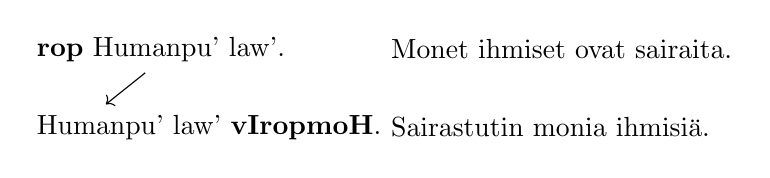
\begin{tikzpicture}
        \node[anchor=west] at (0, 1) {\textbf{rop} Humanpu' law'.};
        \node[anchor=west] at (4.5, 1) {Monet ihmiset ovat sairaita.};
        \draw[->] (1.5, 0.7) -- (1, 0.3);
        \node[anchor=west]  at (0, 0) {Humanpu' law' \textbf{vIropmoH}.};
        \node[anchor=west]  at (4.5, 0) {Sairastutin monia ihmisiä.};
    \end{tikzpicture}
\else
    \begin{tabular}{l l}
        \textbf{rop} Humanpu' law'. & Monet ihmiset ovat sairaita. \\
        Humanpu' law' \textbf{vIropmoH}. & Sairastutin monia ihmisiä. \\
    \end{tabular}
\fi

2. Liitettynä transitiiviseen verbiin \textbf{-moH} merkitsee ''saada joku tekemään''.\\*[1em]
\begin{tabular}{Bl Il | Bl Il}
    ghoj & oppia & ghojmoH & opettaa \\
    ghuH & valmistautua & ghuHmoH & varoittaa \\
    muv & liittyä & muvmoH & rekrytoida \\
    qaw & muistaa & qawmoH & muistuttaa \\
    DoH & perääntyä & DoHmoH & ajaa takaisin \\
\end{tabular}

Alkuperäisen verbin objekti säilyy uuden verbin objektina ja alkuperäisen verbin subjektista tulee uuden verbin epäsuora objekti.

\ifxetex
    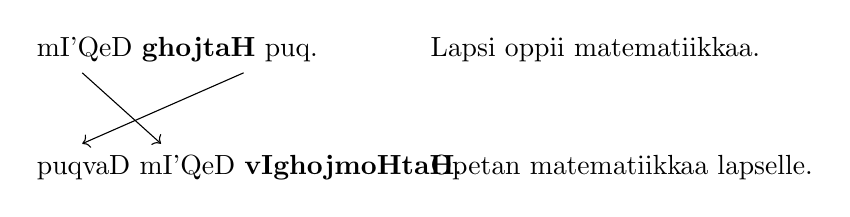
\begin{tikzpicture}
        \node[anchor=west] at (0, 1.5) {mI'QeD \textbf{ghojtaH} puq.};
        \node[anchor=west] at (5, 1.5) {Lapsi oppii matematiikkaa.};
        \draw[->] (2.75, 1.2) -- (0.7, 0.3);
        \draw[->] (0.7, 1.2) -- (1.7, 0.3);
        \node[anchor=west]  at (0, 0) {puqvaD mI'QeD \textbf{vIghojmoHtaH}.};
        \node[anchor=west]  at (5, 0) {Opetan matematiikkaa lapselle.};
    \end{tikzpicture}
\else
    \begin{tabular}{l l}
        mI'QeD \textbf{ghojtaH} puq. & Lapsi oppii matematiikkaa. \\
        puqvaD mI'QeD \textbf{vIghojmoHtaH}. & Opetan matematiikkaa lapselle. \\
    \end{tabular}
\fi

Jos transitiivisella verbillä on refleksiivipääte, se käyttäytyy kuitenkin samoin, kuin intransitiiviset verbit.

\ifxetex
    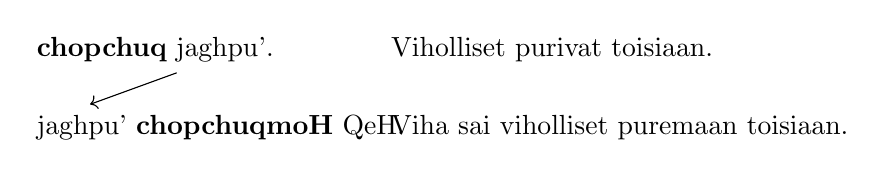
\begin{tikzpicture}
        \node[anchor=west] at (0, 1) {\textbf{chopchuq} jaghpu'.};
        \node[anchor=west] at (4.5, 1) {Viholliset purivat toisiaan.};
        \draw[->] (1.9, 0.7) -- (0.8, 0.3);
        \node[anchor=west]  at (0, 0) {jaghpu' \textbf{chopchuqmoH} QeH.};
        \node[anchor=west]  at (4.5, 0) {Viha sai viholliset puremaan toisiaan.};
    \end{tikzpicture}
\else
    \begin{tabular}{l l}
        \textbf{chopchuq} jaghpu'. & Viholliset purivat toisiaan. \\
        jaghpu' \textbf{chopchuqmoH} QeH. & Viha sai viholliset puremaan toisiaan. \\
    \end{tabular}
\fi

\section{Passiivisuus}\label{sec:passiivi}
\index{passiivi}
\index[sanat]{-lu'}

Passiivin tunnus \textbf{-lu'} merkitsee epämääräistä subjektia.
Verbin persoonapääte valitaan kuin objekti olisi subjekti, mutta objekti kirjoitetaan kuintenkin tavanomaisesti ennen predikaattia.
\index{subjekti}
\index{objekti}\\*[1em]
\begin{tabular}{l l}
    \textbf{vIqawlu'taH}. & Minut muistetaan. \\
    vay' Daja'chugh, \textbf{DaHoHlu'}. & Jos kerrot jollekulle, sinut tapetaan. \\
    roD juHwIj \textbf{Say'moHlu'}. & Kotini siivotaan säännöllisesti. \\
\end{tabular}

Passiivisessa verbissä ei voi käyttää \textbf{-laH}-päätettä.
\index[sanat]{-laH}

Passiivi voi vastata suomen nollapersoonarakennetta, eli jokaisen peräkkäisen passiivisen verbin määrittelemätön tekijä on sama.\\*[1em]
\begin{tabular}{l}
    batlhHa' \textbf{vanglu'taHvIS} quv \textbf{chavbe'lu'}. \\
    Kunniaa ei saa toimimalla epärehellisesti. \\
    \\
    pujwI' \textbf{HIvlu'chugh} \textbf{quvbe'lu'}. \\
    Jos hyökkää heikkoja vastaan ei ole kunniallinen. \\
\end{tabular}

\textbf{tu'}-verbin passiivilla on merkitys \textit{olla jossain}:
\index[sanat]{tu'lu'}\\*[1em]
\begin{tabular}{l l}
    raS DungDaq QIn \textbf{tu'lu'}. & Viesti on pöydän päällä. \\
    DeSwarDaq Sut \textbf{tu'lu'be'}. & Kaapissa ei ole vaatteita. \\
\end{tabular}

\section{-laH-pääte}
\label{sec:laH}
\index[sanat]{-laH}

Modaalinen pääte \textbf{-laH} muuttaa verbin merkitykseksi \textit{voida, osata}.
Se on päätteiden järjestyksessä eri kohdassa kuin muut modaalipäätteet ja sitä ei voi käyttää passiivisissa verbeissä.\\*[1em]
\begin{tabular}{Bl Il}
    -laH & voida, osata \\
    -laHbe' & ei voida, ei osata \\
\end{tabular}

Esimerkiksi:\\*[1em]
\begin{tabular}{l l}
    tlhIngan Hol \textbf{vIjatlhlaHbe'}. & En osaa puhua klingonia. \\
    \textbf{bIQalnISlaH}. & Sinun on osattava uida. \\
    \textbf{lo'laHghach} ghaj'a'? & Onko sillä arvoa? \\
\end{tabular}

\section{Täsmennyspäätteet}
\label{sec:tasmennys}

Täsmennyspäätteillä ilmaistaan kuinka varma puhuja on ja kuinka selvä kuvattu tilanne on.\\*[1em]
\begin{tabular}{Bl Il | Bl Il}
    -chu' & täydellisesti & -chu'be' & epätäydellisesti \\
    -bej & varmasti, kiistatta & -bejbe' & en ole varma \\
    -ba' & selvästi & -ba'be' & ei selvästi \\
    -law' & ilmeisesti & -law'be' & en usko \\
\end{tabular}

\index[sanat]{-chu'}
\textbf{-chu'} merkitsee, että toiminto suoritetaan täydellisesti, virheettä, oikein, täysin tai loppuun asti. Tarkka merkitys riippuu verbistä.\\*[1em]
\begin{tabular}{Bl Il | Bl Il}
    lol & olla ilmassa & lolchu' & olla oikealla korkeudella \\
    nel & sopia & nelchu' & sopia täydellisesti \\
    chuH & heittää keihäs & chuHchu' & osua keihäällä \\
    Suv & taistella & Suvchu' & taistella kuolemaan \\
    HeD & vetäytyä & HeDchu' & vetäytyä kokonaan \\
\end{tabular}

\index[sanat]{-bej}
\textbf{-bej} merkitsee, että lause on kiistattomasti tosi.\\*[1em]
\begin{tabular}{l l}
    \textbf{SuropchoHbej}. & Te sairastutte varmasti. \\
    \textbf{bIlughbejbe'}. & En ole varma, oletko oikeassa. \\
\end{tabular}

\index[sanat]{-ba'}
\textbf{-ba'} merkitsee, että lauseen uskotaan olevan selvästi tosi, mutta se ei ole yhtä kiistatonta kuin \textbf{-bej}-päätteen kanssa.\\*[1em]
\begin{tabular}{l l}
    \textbf{ropba'} ghaH. & Hän on selvästi sairas. \\
    \textbf{bIlughba'be'}. & Ei ole selvää, että olet oikeassa. \\
    \textbf{bIlughbe'ba'}. & Olet selvästi väärässä. \\
\end{tabular}

\index[sanat]{-law'}
\textbf{-law'} merkitsee \textit{uskoa, luulla}:\\*[1em]
\begin{tabular}{l l}
    \textbf{yIropqa'law'}. & Taidan sairastua uudestaan. \\
    \textbf{bIlughlaw'}. & Luulen, että olet oikeassa. \\
    \textbf{bIlughlaw'be'}. & En usko, että olet oikeassa. \\
    \textbf{bIlughbe'law'}. & Luulen, että olet väärässä. \\
\end{tabular}

\section{Aspekti}
\index{aspekti}

Verbin aspekti voidaan ilmaista tarvittaessa seuraavilla päätteillä:\\*[1em]
\begin{tabular}{l Bl l}
    \multirow{2}{*}{imperfektiivinen} & -taH & imperfektiivi \\
    & -lI' & progressiivi \\
    \hline
    \multirow{2}{*}{perfektiivinen} & -pu' & perfektiivi \\
    & -ta' & intentionaali \\
\end{tabular}
\index[sanat]{-taH}
\index[sanat]{-lI'}
\index[sanat]{-pu'}
\index[sanat]{-ta'}
\index{imperfektiivisyys}
\index{perfektiivisyys}

Imperfektiivisyydellä ilmaistaan, että toiminta on jatkuvaa ja päättymätöntä. 
Perfektiivinen toiminta taas on päättynyt.
Toisin kuin suomen kielen perfektiivinen aspekti, klingonin perfektiivinen aspekti ei merkitse toiminnan olevan valmista tai loppuun asti vietyä, vaan toiminta voi olla myös väliaikaisesti keskeytynyt.
Valmista tai loppuun asti vietyä toimintaa ilmaistaan \textbf{-chu'}-päätteellä (ks.~\ref{sec:tasmennys}) tai \textbf{rIntaH}-apuverbillä (ks.~\ref{subsec:rintah}).
Aspektia ei tule sekoittaa aikamuotoihin, joita ei ole klingonissa.

Progressiivinen pääte \textbf{-lI'} merkitsee, että toiminnalla on määränpää tai tavoite (toiminnan ei tarvitse kuitenkaan olla tahallista).
Intentionaalinen pääte \textbf{-ta'} merkitsee, että toiminta on tahallista.
On aina sallittua käyttää näiden päätteiden sijasta vastaavia päätteitä \textbf{-taH} ja \textbf{-pu'}.\\*[1em]
\begin{tabular}{l l}
    \textbf{jISoptaHvIS} yISujQo'. & Älä häiritse minua, kun syön. \\
    \textbf{HeghlI'} ghaH. & Hän on kuolemassa. \\
    qatlh \textbf{DaHoHpu'}? & Miksi tapoit hänet? \\
    \textbf{vIghorta'}. & Rikoin sen tarkoituksella. \\
\end{tabular}
\index{progressiivi}
\index{intentionaali}

Aspektin päätteen liittämistä verbiin, jolla on jussiivin pääte \textbf{-jaj}, tai verbiin, jonka objekti on toinen lause, pidetään huonona kielenkäyttönä. Tämä sääntö ei kuitenkaan ilmeisesti ole aivan ehdoton, sillä sitä on rikottu kaanonissa.
\index[sanat]{-jaj}

\section{-neS-pääte}

\textbf{-neS}-pääte ilmaisee kunnioitusta keskustelun toista osapuolta kohtaan.
Sitä tulee käyttää vain puhuteltaessa ylempiarvoista henkilöä formaalisti.

\textbf{-neSbe'}-päätettä ei ole sopiva käyttää.

\section{Seikkailijat}

Seikkalijat muuttavat niitä edeltävän morfeemin merkitystä.
\index{seikkalija}\\*[1em]
\begin{tabular}{Bl Il}
    -qu' & erittäin \\
    -be' & ei \\
\end{tabular}
\index[sanat]{-qu'}
\index[sanat]{-be'}

Modaalipäätteitä ja täsmennyspäätteitä käsittelevissä luvuissa \ref{sec:modaali}, \ref{sec:laH} ja \ref{sec:tasmennys} on selitetty \textbf{-be'}-päätteen vaikutus näihin päätteisiin.
Muussa tapauksessa \textbf{-be'} kiinnitetään yleensä joko verbin juureen, \textbf{-Ha'}-, \textbf{-choH}-, \textbf{-qa'}-, \textbf{-moH}-, \textbf{-lu'}-päätteeseen tai aspektin päätteeseen riippuen siitä, mikä näistä on viimeinen.

Käskymuotoisissa verbeissä käytetään \textbf{-Qo'}-päätettä \textbf{-be'}-päätteen sijasta.
Jos lauseessa on kielteinen sana, kuten \textbf{pagh}, \textbf{not} tai \textbf{wej}, kieltopäätettä \textbf{be'} ei käytetä.

\textbf{-qu'}-pääte voidaan kiinnittää mihin tahansa morfeemiin lukuunottamatta persoonapäätettä ja myöhemmin tässä luvussa esiteltyjä päätteitä, eli jussiivin, interrogatiivin tai partisiipin tunnusta, konjunktiopäätettä tai substantiivijohdinta.\\*[1em]
\begin{tabular}{l l}
    \textbf{jIropqu'}! & Olen hyvin sairas! \\
    loD \textbf{'IHqu'} vIlegh. & Näin kauniin miehen. \\
\end{tabular}

\section{-Qo'-pääte}
\index[sanat]{-Qo'}

1. \textbf{-Qo'}-päätteellä ilmaistaan kieltäytymistä.\\*[1em]
\begin{tabular}{l l}
    De'wI' Quj \textbf{vIQujQo'}! & En pelaa tietokonepelejä! \\
    Soj tlhol \textbf{SopQo'} puqwI'. & Lapseni ei suostu syömään raakaa \\
    & lihaa. \\
\end{tabular}

2. Imperatiiviverbiin liitettynä \textbf{-Qo'} merkitsee \textit{älä}.
\index{imperatiivi}\\*[1em]
\begin{tabular}{l l}
    \textbf{peqetQo'}! & Älkää juosko! \\
    \textbf{HIquvHa'Qo'}. & Älä häpäise minua! \\
\end{tabular}

\section{Jussiivi}

Jussiivin tunnus \textbf{-jaj} ilmaisee toivetta tai kehoitusta.\\*[1em]
\begin{tabular}{l l}
    \textbf{taHjaj} tlhIngan wo'! & Eläköön klingonien valtakunta! \\
\end{tabular}

\section{Interrogatiivi}
\index{interrogatiivi}

Interrogatiivi eli kysymysmuoto muuttaa lauseen kysymykseksi.
Interrogatiivin tunnus on \textbf{-'a'}.
\index[sanat]{-'a'}\\*[1em]
\begin{tabular}{l l}
    nIm Datlhutlh\textbf{'a'}? & Juotko maitoa? \\
    tlhIngan Hol Dajatlh\textbf{'a'}? & Puhutko klingonia? \\
\end{tabular}

Interrogatiivia ei käytetä, jos lauseessa on kysymyssana.\\*[1em]
\begin{tabular}{l l}
    \textbf{nuq} Datlhutlh? & Mitä juot? \\
    \textbf{qatlh} tlhIngan Hol Dajatlh? & Miksi puhut klingonia? \\
\end{tabular}

Lauseen voi muuttaa kysymykseksi myös sanalla \textbf{qar'a'} \textit{vai mitä}.

\section{Konjunktiopäätteet}
\label{sec:konjunktiopaate}
\index{konjunktiopääte}

Konjunktiopäätteet kiinnitetään sivulauseen predikaattiin.\\*[1em]
\begin{tabular}{Bl Il}
    -vIS & kun \\
    -DI' & heti kun \\
    -pa' & ennen kun \\
    -chugh & jos \\
    -mo' & koska \\
    -meH & jotta \\
\end{tabular}
\index[sanat]{-vIS}
\index[sanat]{-DI'}
\index[sanat]{-pa'}
\index[sanat]{-chugh}
\index[sanat]{-mo'}
\index[sanat]{-meH}

\textbf{-vIS}-päätteen kanssa on käytettävä imperfektiivistä aspektia (\textbf{-taH}).\\*[1em]
\begin{tabular}{l l}
    bIropchoH\textbf{chugh}, jImej. & Lähden, jos sairastut. \\
    bItuSchoH\textbf{DI'}, jIqet. & Juoksen heti kun alat yskimään. \\
    jIqettaH\textbf{vIS}, 'oy' 'uSDu'wIj. & Jalkoihini sattuu, kun juoksen. \\
    jIHoSmoH\textbf{meH}, jISuv. & Taistelen voimistuakseni. \\
    bIQob\textbf{mo'}, yIngab! & Koska olet vaarallinen, katoa! \\
    bIchegh\textbf{pa'}, yIQub! & Mieti ennen kun palaat! \\
\end{tabular}

\textbf{-meH}-päätteinen verbi voi määrittää lauseen lisäksi myös substantiivia.\\*[1em]
\begin{tabular}{l l Il}
    \textbf{DIlmeH} Huch & ''raha maksamiseen'' & hinta \\
    \textbf{ghojmeH} paq & ''kirja oppimiseen'' & oppikirja \\
    \textbf{HIjmeH} chaw' & ''lupa toimittamiseen'' & postimerkki \\
    \textbf{ngongmeH} Duj & ''alus testaamiseen'' & koealus \\
\end{tabular}

\textbf{-meH}-päätettä käytetään sanan \textbf{Qu'} \textit{tehtävä} kanssa, kun lauseen halutaan olevan toisen lauseen subjekti.\\*[1em]
\begin{tabular}{l l}
    Qatlh jagh leghmeH \textbf{Qu'}. & Vihollisen näkeminen on vaikeaa. \\
    jIHvaD potlh SuvmeH \textbf{Qu'}. & Taisteleminen on minulle tärkeää. \\
\end{tabular}

\section{Partisiipit}
\index{partisiippi}

Partisiippi muodostetaan verbistä \textbf{-bogh}-päätteellä.
Partisiippi ei ole adjektiivi, vaan se sijoitetaan joko ennen tai jälkeen pääsanaansa riippuen siitä, onko pääsana verbin subjekti vai objekti.
\index[sanat]{-bogh}

Aktiivin partisiippi sijoitetaan ennen pääsanaansa.
Tällöin pääsana on partisiipin subjekti.
Passiivin partisiippi taas sijoitetaan pääsanansa jälkeen, jolloin pääsana on partisiipin objekti.\\*[1em]
\begin{tabular}{l l}
    \textbf{Qapbogh} SuvwI' & onnistunut soturi \\
    SuvwI' \textbf{jeybogh} & voitettu soturi \\
\end{tabular}

Partisiipilla voi olla sekä subjekti tai objekti.
Jos pääsana on partisiipin objekti, sen on oltava \textbf{-'e'}-sijassa.
Jos taas pääsana on partisiipin subjekti, se voi olla \textbf{-'e'}-sijassa.\\*[1em]
\begin{tabular}{l l}
    jagh \textbf{jeybogh} SuvwI' / SuvwI''e' & vihollisen voittanut soturi \\
    SuvwI''e' \textbf{jeybogh} jagh & vihollisen voittama soturi \\
\end{tabular}

\section{Substantiivijohtimet}
\index{substantiivijohdin}

\textbf{-wI'}-johdin vastaa suomen \textit{-ja}-johdinta.
Se muuttaa verbin subjektia vastaavaksi substantiiviksi.
\index[sanat]{-wI'}\\*[1em]
\begin{tabular}{Bl Il | Bl Il}
    ghoj & oppia & ghojwI' & oppilas \\
    ghojmoH & opettaa & ghojmoHwI' & opettaja \\
    nep & valehdella & nepwI' & valehtelija \\
    chIS & olla valkoinen & chISwI' & valkoinen \\
    po' & olla taitava & po'wI' & asiantuntija \\
    ngaQHa'moH & poistaa lukitus & ngaQHa'moHwI' & avain \\
\end{tabular}

\textbf{-ghach}-johdin muuttaa verbin abstraktiksi substantiiviksi.
\index[sanat]{-ghach}\\*[1em]
\begin{tabular}{Bl Il | Bl Il}
    lo'laH & voida käyttää & lo'laHghach & arvo \\
    quvHa' & olla häpäisty & quvHa'ghach & häpeä \\
    bomlaH & voida laulaa & bomlaHghach & laulutaito \\
    wovtaH & olla kirkas & wovtaHghach & kirkkaus \\
    nIv & olla suuremmoinen & nIvghach & suuremmoisuus \\
\end{tabular}

\textbf{-ghach}-johtimen liittämistä verbiin, jolla ei ole yhtään päätettä tai johtinta, pidetään huonona tai korosteisena kielenkäyttönä. Alla on korvaavia rakenteita.

1. monet verbit sellaisenaan ovat substantiiveja ilman johdinta\\*[1em]
\begin{tabular}{Bl Il | Bl Il}
    quv & kunnioittaa & quv & kunnia \\
    bom & laulaa & bom & laulu \\
    bel & nauttia & bel & nautinto \\
\end{tabular}

2. \textbf{-meH}-pääte + substantiivi (ks.~\ref{sec:konjunktiopaate})\\*[1em]
\begin{tabular}{Bl Il | Bl Il}
    tlhuH & hengittää & tlhuHmeH Qu' & hengittäminen \\
    qaHoH & tapan sinut & qaHoHmeH Qu' & sinun tappamisesi \\
    wIghoS & tulemme & wIghoSmeH ngoQmaj & tulemisemme syy \\
\end{tabular}

\section{Apuverbit}
\index{apuverbi}

\subsection{neH}
\index[sanat]{neH}

Apuverbin \textbf{neH} \textit{haluta} kanssa ei käytetä relatiivipronominia \textbf{'e'}. \\*[1em]
\begin{tabular}{l l}
    jISuv \textbf{vIneH}! & Haluan taistella! \\
\end{tabular}

\subsection{qa'}
\index[sanat]{qa'}

Apuverbiä \textbf{qa'} \textit{korvata} käytetään \textit{jonkin sijasta} -rakenteessa. Relatiivipronomini \textbf{'e'} on valinnainen.\\*[1em]
\begin{tabular}{l l}
    vIghro' vISuqnIS. yIH \textbf{qa'}. & Minun on hankittava kissa tribblen tilalle. \\
    juHDaq jIba'. jIqet ('e') \textbf{qa'}. & Istun kotona juoksemisen sijaan. \\
\end{tabular}

\subsection{rIntaH}
\label{subsec:rintah}
\index[sanat]{rIntaH}

Apuverbi \textbf{rIntaH} merkitsee, että jokin on tapahtunut, lopullinen. Se on taipumaton.\\*[1em]
\begin{tabular}{l l}
    Heghpu' \textbf{rIntaH} jaghwI'. & Viholliseni on kuollut (lopullisesti). \\
    bIquvHa'choHta' \textbf{rIntaH}. & Olet ikuisessa häpeässä. \\
\end{tabular}

\subsection{jalchugh}
\index[sanat]{jalchugh}

Rakenne \textbf{net jalchugh} \textit{jos kuvitellaan, että} vastaa suomen konditionaalia.\\*[1em]
\begin{tabular}{l l}
    nuH vIghaj \textbf{net jalchugh}, vaj jIHIv. & Jos minulla olisi ase, niin hyökkäisin. \\
    bIropbe' \textbf{net jalchugh}, qaSuchbej. & Jos et olisi sairas, tulisin varmasti \\ & tapaamaan sinua. \\
\end{tabular}

\section{Vertailuverbit}
\label{sec:vertailuverbit}
\index{vertailuverbi}
\index[sanat]{rur}
\index[sanat]{rap}
\index[sanat]{nIb}

\begin{tabular}{Bl Il}
    rur & muistuttaa \\
    rap & olla samanlainen \\
    nIb & olla identtinen \\
\end{tabular}

Vertailuverbejä käytetään suomen kielen \textit{kuin}-sanan tapaan.\\*[1em]
\begin{tabular}{l l}
    'IH naghbochvam; Har'ey \textbf{rur}. & Tämä jalokivi on kaunis kuin sateenkaari. \\
    yItlh ghojmoHwI'; \textbf{rap} qaytu'pu'wI'. & Opettaja oli yhtä ankara kuin vanhempani. \\
    tIq tajlIj; \textbf{nIb} naQjejHomvetlh. & Veitsesi on yhtä pitkä kuin tuo nuoli. \\
\end{tabular}

\textbf{nIb} eroaa \textbf{rap}-sanasta siten, että \textbf{nIb} antaa ymmärtää jonkin vertailtavien asioiden mitattavan suureen olevan täsmälleen sama.

\chapter{Pronominit}

\section{Persoonapronominit}
\index{persoonapronomini}
\index[sanat]{jIH}
\index[sanat]{maH}
\index[sanat]{SoH}
\index[sanat]{tlhIH}
\index[sanat]{ghaH}
\index[sanat]{chaH}
\index[sanat]{'oH}
\index[sanat]{bIH}

Klingonissa on seuraavat persoonapronominit:\\*[1em]
\begin{tabular}{l Bc Bc}
    persoona & \multicolumn{1}{c}{yksikkö} & \multicolumn{1}{c}{monikko} \\
    1. & jIH & maH \\
    2. & SoH & tlhIH \\
    3., henkilöt & ghaH & chaH \\
    3., muut & 'oH & bIH \\
\end{tabular}

Pronominit toimivat substantiivin tavoin ja niitä voi taivuttaa sijamuodoissa.
Pronomineja ei kuitenkaan voi käyttää ilmaisemaan omistamista, vaan siihen käytetään erillisiä omistusliitteitä.\\*[1em]
\begin{tabular}{l l}
    \textbf{ghaH} yIQaH! & Auta häntä! \\
    \textbf{jIHvaD} 'oH yInobHa'. & Palauta se minulle. \\
\end{tabular}

Persoonapronomini voi toimia verbinä, jolloin sen merkitys on \textit{olla}.
Tällöin pronomini voi ottaa verbipäätteitä, mutta ei persoonaetuliitettä.
\index{olla-verbi}\\*[1em]
\begin{tabular}{l l}
    tlhIngan \textbf{jIHbe'}. & En ole klingoni.\\
    'Iv \textbf{maH}? & Keitä me olemme? \\
\end{tabular}

\section{Interrogatiivipronominit}
\index{interrogatiivipronomini}
\index[sanat]{nuq}
\index[sanat]{'Iv}

Interrogatiivipronominit ovat kysymyssanoina toimivia pronomineja.\\*[1em]
\begin{tabular}{Bl Il}
    nuq & mikä \\
    'Iv & kuka \\
\end{tabular}

\textbf{'Iv}-pronominia käytetään henkilöiden kanssa ja \textbf{nuq}-proniminia muiden sanojen kanssa.

Esimerkiksi:\\*[1em]
\begin{tabular}{l l}
    DughIj \textbf{nuq}? & Mikä pelottaa sinua? \\
    lugh \textbf{'Iv}? & Kuka on oikeassa? \\
\end{tabular}

Kuten persoonapronominitkin, interrogatiivipronominit voivat toimia verbinä ja niitä voi taivuttaa sijamuodoissa.\\*[1em]
\begin{tabular}{l l}
    ghojmoHwI'lI' \textbf{'Iv}? & Kuka on opettajasi? \\
    \textbf{'IvvaD} DangeH? & Kenelle lähetät sen? \\
    \textbf{nuqDaq} bIjaH? & Minne menet? \\
\end{tabular}

\section{Indefiniittipronominit}

\subsection{Kvanttoripronominit}
\index{kvanttoripronomini}
\index[sanat]{pagh}
\index[sanat]{vay'}
\index[sanat]{'op}
\index[sanat]{ngIq}
\index[sanat]{Hoch}

Klingonissa on seuraavat kvanttoripronominit:\\*[1em]
\begin{tabular}{Bl l}
    pagh & \textit{ei kukaan, ei mikään} \\
    vay' & \textit{joku, jokin} \\
    'op & (laskettaville sanoille:) \textit{jotkut}; (ainesanoille:) \textit{vähän, jonkin verran} \\
    ngIq & \textit{yksittäinen}; \textit{yksi kerrallaan} \\
    Hoch & \textit{jokainen, kaikki} \\
\end{tabular}

Esimerkiksi:\\*[1em]
\begin{tabular}{l l}
    ropchoH, neH \textbf{pagh}. & Kukaan ei halua sairastua. \\
    tlhoy Sop \textbf{vay'}. & Joku söi liikaa. \\
    ru' \textbf{Hoch}. & Kaikki on väliaikaista. \\
\end{tabular}

\textbf{pagh} ja \textbf{Hoch} voivat toimia substantiivin määreinä. \textbf{'op} esiintyy vain substantiivin määreenä.\\*[1em]
\begin{tabular}{l l}
    'oH Sov \textbf{Hoch} tlhIngan. & Sen tietää jokainen klingoni. \\
    mutlhej \textbf{pagh} jatlhwI'. & Minulla ei ole ketään kelle puhua. \\
    \textbf{'op} HIq vItlhutlh neH! & Minä vain join vähän viiniä! \\
    mupar \textbf{'op} Qel. & Jotkut lääkärit vihaavat minua. \\
\end{tabular}

\textbf{ngIq} voi toimia substantiivin määreenä. Riippuen asiayhteydestä se voi viitata joko yksittäiseen asiaan sarjassa tai kaikkiin sarjan asioihin.\\*[1em]
\begin{tabular}{l l}
    \textbf{ngIq} jupwI' vIqan. & Tervehdin yksi kerrallaan ystäviäni. \\
    \textbf{ngIq} tonSaw lo' 'ej Quj Qap. & Hän voitti pelin yhdellä siirrolla. \\
\end{tabular}

\subsection{Pronomini latlh}
\index[sanat]{latlh}

Indefiniittipronomini \textbf{latlh} merkitsee \textit{toinen}.
\index{indefiniittipronomini}

\section{Relatiivipronominit}
\index{relatiivipronomini}
\index[sanat]{'e'}
\index[sanat]{net}

Klingonissa on kaksi relatiivipronominia: \textbf{'e'} ja \textbf{net}.
Molemmat viittaavat edeltävään lauseeseen.

\textbf{'e'} merkitsee \textit{se, että}.\\*[1em]
\begin{tabular}{l l}
    Qatlh veS, \textbf{'e'} vISov. & Tiedän, että sota on vaikeaa. \\
    bISuv \textbf{'e'} lulegh. & He näkevät, että olet taistelet. \\
    vaj yInlu' \textbf{'e'} toblu'. & Niin todistaa, että elää. \\
\end{tabular}

\textbf{net} muuttaa lauseen merkityksen passiiviseksi.\\*[1em]
\begin{tabular}{l l}
    Qatlh veS, \textbf{net} Sov. & Tiedetään, sota on vaikeaa. \\
    bISuv \textbf{net} legh. & Taistelemisesi nähdään. \\
    yInlu' \textbf{net} tob. & Todistetaan elämistä. \\
\end{tabular}

\textbf{'e'}-pronominia ei käytetä \textbf{neH}-apuverbin kanssa.
\index[sanat]{neH}\\*[1em]
\begin{tabular}{l l}
    jIropHa'choH \textbf{vIneH}. & Haluan parantua. \\
    ghorgh bIQongchoH \textbf{DaneH?} & Milloin haluat mennä nukkumaan? \\
\end{tabular}

\chapter{Adverbit}
\index{adverbi}

Lista yleisimmistä adverbeista on liitteessä~\ref{apx:adverbit}.

\section{Adverbien sijainti}

Yleensä adverbit sijoitetaan lauseen alkuun.\\*[1em]
\begin{tabular}{l l}
    \textbf{nom} jIqet. & Juoksen nopeasti. \\
    \textbf{wa'leS} ghaH vIlegh. & Näin hänet eilen. \\
    \textbf{chaq} jIlughbe'. & Ehkä olen väärässä. \\
    \textbf{qatlh} DaHoH? & Miksi tapoit hänet? \\
\end{tabular}

\section{Adverbit je, neH ja neHHa'}
\index[sanat]{je}
\index[sanat]{neH}
\index[sanat]{neHHa'}

Poikkeuksellisesti adverbit \textbf{je} \textit{myös}, \textbf{neH} \textit{vain}, \textbf{neHHa'} \textit{ei vain} sijoitetaan predikaatin jälkeen.\\*[1em]
\begin{tabular}{l l}
    bIropchoH \textbf{je} vIneHbe'! & En halua, että lisäksi sairastut! \\
    ghaHvaD jIjatlhlaHchugh \textbf{neH}... & Jos vain voisin puhua hänelle... \\
\end{tabular}

\textbf{je}, \textbf{neH} ja \textbf{neHHa'} voivat toimia myös adjektiivin tavoin substantiivin tai pronominin määreinä.\\*[1em]
\begin{tabular}{l l}
    tlhIngan Hol \textbf{je} vIjatlh. & Puhun myös klingonia. \\
    Soj tlhol \textbf{neH} vISop. & Syön vain raakaa ruokaa. \\
\end{tabular}

%\section{Adverbi jay'}
% Tämä on kirosana, joten kuuluuko sitä käsitellä "lukion" kielioppikirjassa?

\section{Adverbit law' ja puS}
\index[sanat]{law'}
\index[sanat]{puS}

Adverbeja \textbf{law'} \textit{paljon} ja \textbf{puS} \textit{vähän} käytetään vertailurakenteissa.
\index{vertailurakenne}\\*[1em]
\begin{tabular}{l l}
    jIH HoS \textbf{law'}, SoH HoS \textbf{puS}. & Olen sinua voimakkaampi. \\
    ghaH po' \textbf{law'be'}, jIH po' \textbf{puSbe'}. & Hän ei ole minua taitavampi. \\
    DujlIj 'IH \textbf{law'}, DujwIj 'IH \textbf{law'}. & Aluksesi on yhtä kaunis kuin minun. \\
\end{tabular}

Superlatiivirakenteessa käytetään sanaa \textbf{Hoch} \textit{kaikki}.
\index{superlatiivi}
\index[sanat]{Hoch}\\*[1em]
\begin{tabular}{l l}
    ghaH mIp \textbf{law'}, \textbf{Hoch} mIp \textbf{puS}. & Hän on rikkain. \\
    Duj'e', 'oH wagh \textbf{law'}, \textbf{Hoch} wagh \textbf{puS}. & Se on kallein alus. \\
\end{tabular}

\section{Paikka-adverbeja}
\index{paikka-adverbi}
\index[sanat]{Dat}
\index[sanat]{vogh}
\index[sanat]{naDev}
\index[sanat]{pa'}

Substantiiveja \textbf{Dat} \textit{kaikkialla}, \textbf{vogh} \textit{jossain}, \textbf{naDev} \textit{täällä} ja \textbf{pa'} \textit{siellä} ei voi taivuttaa lokatiivissa.
Sen sijasta ne toimivat sellaisenaan adverbeina.\\*[1em]
\begin{tabular}{Bl Il | r Bl Il l}
    Dat & kaikkialla & ( & Datvo' & kaikkialta & ) \\
    vogh & jossain & ( & voghvo' & jostain & ) \\
    naDev & täällä & ( & naDevvo' & täältä & ) \\
    pa' & siellä & ( & pa'vo' & sieltä & ) \\
\end{tabular}

Sanalla \textbf{pa'} on myös merkitys \textit{huone}.
Tällöin se taipuu normaalisti lokatiivissa.\\*[1em]
\begin{tabular}{l l}
    \textbf{pa'} vIQong. & Nukuin siellä. \\
    \textbf{pa'Daq} vIQong. & Nukuin huoneessa. \\
\end{tabular}

\section{Laskuriadverbit}
\index{laskuriadverbi}
\index[sanat]{leS}
\index[sanat]{Hu'}
\index[sanat]{wen}
\index[sanat]{waQ}
\index[sanat]{ben}
\index[sanat]{nem}
\index[sanat]{ret}
\index[sanat]{pIq}

Laskuriadverbit seuraavat lukumäärää ja ilmaisevat ajan kulumista.\\*[1em]
\begin{tabular}{Bl Il}
    Hu' & päivää sitten \\
    leS & päivän päästä \\
    wen & kuukautta sitten \\
    waQ & kuukauden päästä \\
    ben & vuotta sitten \\
    nem & vuoden päästä \\
    ret & (ajanyksikköä) sitten \\
    pIq & (ajanyksikön) päästä \\
\end{tabular}

Esimerkkejä:\\*[1em]
\begin{tabular}{l l}
    cha'maH \textbf{ben} jIbogh. & Olen kaksikymmentä vuotta vanha. \\
    wa'\textbf{leS} jISuvbe'. & En taistellut eilen. \\
    wej \textbf{wen} bIropchoH. & Sairastuit kolme kuukautta sitten. \\
    wa' \textbf{nem} mamIp. & Vuoden päästä olemme rikkaita. \\
\end{tabular}

\textbf{ret} ja \textbf{pIq} seuraavat lukumäärää ja yksikköä.\\*[1em]
\begin{tabular}{l l}
    cha' \textbf{rep ret} Hegh. & Hän kuoli kaksi tuntia sitten. \\
    wa'maH \textbf{lup pIq} maHIv. & Hyökkäämme kymmenen sekunnin kuluttua. \\
\end{tabular}

\section{Interrogatiiviadverbit}
\index[sanat]{chay'}
\index[sanat]{ghorgh}
\index[sanat]{qatlh}
\index[sanat]{'ar}
\index[sanat]{'arlogh}

\begin{tabular}{Bl Il}
    chay' & miten \\
    ghorgh & milloin \\
    qatlh & miksi \\
    'ar & kuinka monta / paljon \\
    'arlogh & kuinka monta kertaa \\
\end{tabular}

\textbf{'ar} seuraa substantiivia. Tällöin substantiivin kanssa ei käytetä monikkoliitettä.\\*[1em]
\begin{tabular}{l l}
    paq \textbf{'ar} Daghaj? & Kuinka monta kirjaa sinulla on? \\
    yuch \textbf{'ar} DaSop DaneH? & Kuinka paljon suklaata haluat syödä? \\
    ben \textbf{'ar} bIboghpu'? & Kuinka monta vuotta sitten synnyit? \\
\end{tabular}

\chapter{Konjunktiot}

\section{'ej, qoj, pagh}
\index[sanat]{'ej}
\index[sanat]{qoj}
\index[sanat]{pagh}

Seuraavat konjunktiot erottavat lauseita, partisiippeja ja adverbeja toisistaan.\\*[1em]
\begin{tabular}{Bl Il}
    'ej & ja \\
    qoj & ja/tai \\
    pagh & joko ... tai \\
\end{tabular}

Esimerkiksi:\\*[1em]
\begin{tabular}{l l}
    Sopbe' \textbf{'ej} tlhutlhbe' qoqmey. & Robotit eivät syö eivätkä juo. \\
    HoSbogh \textbf{'ej} Qupbogh SuvwI' yoH & rohkea, voimakas ja nuori soturi \\
    taH \textbf{pagh} taHbe'. & Ollako vai eikö olla. \\
\end{tabular}

\section{je, joq, ghap}
\index[sanat]{je}
\index[sanat]{joq}
\index[sanat]{ghap}

Nämä konjunktiot erottavat substantiivilausekkeista toisistaan.\\*[1em]
\begin{tabular}{Bl Il}
    je & ja \\
    joq & ja/tai \\
    ghap & joko ... tai \\
\end{tabular}

Esimerkiksi:\\*[1em]
\begin{tabular}{l l}
    juHqo' miDmey \textbf{je} wIHub. & Puolustamme kotimaailmaa ja siirtokuntia. \\
\end{tabular}

\textbf{je} merkitsee \textit{myös}, jos sitä edeltää vain yksi substantiivilauseke.

\chapter{Numeraalit}
\index{numeraali}

Klingonin lukusanat muodostetaan kymmenjärjestelmän numeroista ja suuruusluokkaa kuvaavista liitteistä.
\index{lukusana}\\*[1em]
\begin{tabular}{Bl Il | Bl Il}
    pagh & nolla & -maH & kymmenen \\
    wa' & yksi & -vatlh & sata \\
    cha' & kaksi & -SaD/-SanID & tuhat \\
    wej & kolme & -netlh & kymmenen tuhatta \\
    loS & neljä & -bIp & sata tuhatta \\
    vagh & viisi & -'uy' & miljoona \\
    jav & kuusi & -vatlhbIp/-maH'uy' & kymmenen miljoonaa \\
    Soch & seitsemän & -Sa(nI)DbIp/-vatlh'uy' & sata miljoonaa \\
    chorgh & kahdeksan & -Saghan & miljardi \\
    Hut & yhdeksän & & \\
\end{tabular}
\index[sanat]{-maH}
\index[sanat]{-vatlh}
\index[sanat]{-SaD}
\index[sanat]{-SanID}
\index[sanat]{-netlh}
\index[sanat]{-bIp}
\index[sanat]{-'uy'}

Luku esitetään merkitsevin numero ensin kuten suomessakin.
Sanaa \textbf{pagh} \textit{nolla} käytetään vain yksin eikä siihen saa liittää suurusluokkaliitteitä.
\index[sanat]{pagh}

Suurille luvuille ei ole omia liitteitä, vaan niille voi käyttää yhdistelmiä, esimerkiksi \textit{kymmenelle miljoonalle} voi käyttää liiteitä \textbf{-vatlhbIp} \textit{sata sataa tuhatta} tai \textbf{-maH'uy'} \textit{kymmenen miljoonaa}.

Esimerkiksi luku 103 621 esitetään seuraavasti:\\*[1em]
\begin{tabular}{c c c c c c}
    \textbf{wa'bIp} & & \textbf{wejSaD} & \textbf{javvatlh} & \textbf{cha'maH} & \textbf{wa'} \\
    1 & 0 & 3 & 6 & 2 & 1 \\
    \multicolumn{6}{c}{satakolmetuhattakuusisataakaksikymmentäyksi} \\
\end{tabular}

Luku kirjoitetaan yleensä ennen pääsanaansa.\\*[1em]
\begin{tabular}{l l}
    \textbf{cha'} SuvwIpu' & kaksi soturia \\
    Hoch rewbe' QaH \textbf{wa'} mang. & Yksi sotilas auttaa kaikkia \\
    & kansalaisia. \\
\end{tabular}

Luvusta voi tehdä järjestysluvun \textbf{-DIch}-johtimella.
Järjestysluvut kirjoitetaan adjektiivin tavoin pääsanansa jälkeen.
\index[sanat]{-DIch}
\index{järjestysluku}\\*[1em]
\begin{tabular}{l l}
    \textbf{wa'DIch} & \textit{ensimmäinen} \\
    \textbf{cha'DIch} & \textit{toinen} \\
    \textbf{wa'maHDIch} & \textit{kymmenes} \\
    veng \textbf{wa'DIch} & Ensimmäinen Kaupunki \\
    \textbf{wa'DIch} jISop. & Syön ensin. \\
\end{tabular}

\textbf{-logh}-johdin muuttaa luvun adverbiksi, jolla on merkitys \textit{kertaa}.
\index[sanat]{-logh}\\*[1em]
\begin{tabular}{Bl Il}
    paghlogh & ei kertaakaan \\
    wa'logh & kerran \\
    cha'logh & kahdesti, kaksi kertaa \\
\end{tabular}

\appendix
\chapter{Klingonin aakkoset}

\begin{tabular}{Tl Bl Il | Tl Bl Il | Tl l Il}
     & a & 'at &  & o & 'ot &  & 0 & pagh \\
     & b & bay &  & p & pay &  & 1 & wa' \\
     & ch & chay &  & q & qay &  & 2 & cha' \\
     & D & Day &  & Q & Qay &  & 3 & wej \\
     & e & 'et &  & r & ray &  & 4 & loS \\
     & gh & ghay &  & S & Say &  & 5 & vagh \\
     & H & Hay &  & t & tay &  & 6 & jav \\
     & I & 'It &  & tlh & tlhay &  & 7 & Hoch \\
     & j & jay &  & u & 'ut &  & 8 & chorgh\\
     & l & lay &  & v & vay &  & 9 & Hut\\
     & m & may &  & w & way & & & \\
     & n & nay &  & y & yay &  & , & \\
     & ng & ngay &  & ' & qaghwI' &  & . & \\
\end{tabular}

Yllä olevassa taulukossa on listattu klingonin romanisaation ''aakkoset'' ja yleiset tavat niiden lausuminen sanojen tavaamista varten.
Taulukossa merkityt grafeemit eivät oikeastaan ole aakkosia (ne koostuvat latinalaisista aakkosista), mutta niistä puhutaan usein ''kirjaimina'' tai ''aakkosina''.
Ne myös käyttäytyvät kuten aakkoset siinä mielessä,
että yleisen tavan mukaan esimerkiksi \textbf{ng}:llä alkavat sanat aakkostetaan sanakirjassa vasta kaikkien \textbf{n}:llä alkavien sanojen jälkeen.
Kolmannessa sarakkeessa olevat ääntämisohjeet eivät siis ole aakkosten nimiä, vaan oikeastaan äänteiden nimiä.

Ensimmäiseen sarakkeeseen merkityt ''pIqaD-merkit'' perustuvat Star Trek -sarjoissa ja elokuvissa nähtyihin koristeellisiin merkkeihin.
Star Trekissä nämä merkit eivät siis alunperin tarkoittaneet mitään (kuten ei sarjojen ''klin\-gon\-kaan'').
Myöhemmin tuntemattomaksi jääneet henkilöt yhdistivät merkit romanisaation grafeemeihin luoden uuden ''fanikirjoitusjärjestelmän'',
joka on sitemmin saavuttanut suuren suosion klingon-harrastajien keskuudessa.
Tätä ''pIqaDia'' ei kuitenkaan voida pitää mitenkään kanonisena tai virallisena tapana kirjoittaa klingonia.

\chapter{Oikeinkirjoitus}

Tämä luku käsittelee klingonin romanisaation oikeinkirjoitusta.
pIqaD-järjestelmää ei käsitellä.

\section{Isot ja pienet kirjaimet}

Standardiromanisaatiossa erikokoisten kirjainten ajatellaan olevan eri merkkejä.
Kirjaimet \textbf{D}, \textbf{H}, \textbf{I} ja \textbf{S} kirjoitetaan aina isolla kirjaimella.
Kirjaimet \textbf{Q} ja \textbf{q} ovat erilliset kirjaimet ja ne äännetään eri tavoin.
Kaikki muut kirjaimet kirjoitetaan pienellä.
\footnote{
    Syy tälle käytännölle on, että romanisaatiossa halutaan huomioida eri murteiden erilaiset ääntämisasut, minkä vuoksi on tarvittu enemmän merkkejä kuin mitä englannin aakkostossa on.
    Siksi isoja ja pieniä aakkosia käytetään eri äänteiden merkitsemiseen, esimerkiksi \textbf{h} /h/ ja \textbf{H} /χ/.
    Standardiklingonissa ei kuitenkaan käytetä kaikkia näitä äänteitä, mikä selittää romanisaation näennäisen epäjohdonmukaisuuden.
}

\section{Pilkutus}

Romanisaatiossa noudatetaan melko vapaita pilkutussääntöjä.
Pilkkua voidaan käyttää tarvittaessa erottamaan

1. päälausetta ja päälausetta

2. sivulausetta ja päälausetta

3. objektia ja predikaattia

4. listan osia

Vertailuverbit (\textbf{rur}, \textbf{rap}, \textbf{nIb}) erotetaan edeltävästä lauseesta puolipisteellä, kun niitä käytetään suomen kielen \textit{kuin}-sanaa vastaavalla tavalla (ks. \ref{sec:vertailuverbit}).

\section{Yhdyssanat ja sanaliitot}

Erikseen kirjoitetaan aina

1. \textbf{-meH}-päätteen sisältävät sanaliitot\\*[1em]
\begin{tabular}{Bl Il}
    ghojmeH paq & oppikirja \\
\end{tabular}

2. \textbf{qach}-loppuiset sanaliitot\\*[1em]
\begin{tabular}{Bl Il}
    juH qach & kotitalo \\
    much qach & teatteri \\
    ropyaH qach & sairaala \\
\end{tabular}

poikkeus:\\*[1em]
\begin{tabular}{Bl Il}
    chalqach & torni \\
\end{tabular}

Yhteen kirjoitetaan aina

1. \textbf{-ngan}-loppuiset yhdyssanat\\*[1em]
\begin{tabular}{Bl Il}
    tera'ngan & maan asukas \\
    tlhIngan & klingoni \\
\end{tabular}

2. \textbf{-SIp}-loppuiset yhdyssanat\\*[1em]
\begin{tabular}{Bl Il}
    bIQSIp & vety \\
    julSIp & helium \\
    yInSIp & happi \\
\end{tabular}

3. \textbf{-QeD}-loppuiset yhdyssanat, jos alkuosa ei ole sanaliitto\\*[1em]
\begin{tabular}{Bl Il}
    HolQeD & kielitiede \\
    mI'QeD & matematiikka \\
    tamlerQeD & kemia \\
\end{tabular}

poikkeus:\\*[1em]
\begin{tabular}{Bl Il}
    DI'ruj QeD & metafysiikka \\
\end{tabular}

4. \textbf{-tej}-loppuiset yhdyssanat\\*[1em]
\begin{tabular}{Bl Il}
    Holtej & kielitieteilijä \\
    tamlertej & kemisti \\
    'otlhtej & kvanttitieteilijä \\
\end{tabular}

poikkeus:\\*[1em]
\begin{tabular}{Bl Il}
    mI' tej & matemaatikko \\
\end{tabular}

5. eräät adverbit\\*[1em]
\begin{tabular}{Bl Il}
    DaHjaj  & tänään \\
    wa'Hu' & eilen \\
    wa'leS & huomenna \\
\end{tabular}

Muistattava yksitellen:

1. huoneiden nimet (\textbf{pa'}-loppuiset sanaliitot ja yhdyssanat)\\*[1em]
\begin{tabular}{Bl Il}
    jonta' pa' & konehuone \\
    bo'DIj pa' & oikeussali \\
    Qulpa' & laboratorio \\
    puchpa' & kylpyhuone \\
\end{tabular}

2. alusten nimet (\textbf{Duj}-loppuiset sanaliitot ja yhdyssanat)\\*[1em]
\begin{tabular}{Bl Il}
    bIQ Duj & vene, laiva \\
    chach Duj & hätätila-ajoneuvo, ambulanssi \\
    puH Duj & auto \\
    tut Duj & hissi \\
    toDDuj & pelastusalus \\
    SuyDuj & kauppa-alus \\
    veSDuj & sota-alus \\
\end{tabular}

\chapter{Klingonin fonotaksi}
\label{apx:fonotaksi}

Fonotaksi tarkoittaa niitä sääntöjä, joiden mukaan äänteitä saa yhdistellä ja tavuja rakentaa.

Klintonin sanat koostuvat \textbf{tavuista}.
Tavu on joko muotoa KV, KVK tai KVY, missä K on konsonantti, V vokaali ja Y konsonanttiyhdistelmä.

\textbf{Konsonantteja} ovat:\\*[1em]
b ch D gh H j l m n ng p q Q r S t tlh v w y '

\textbf{Vokaaleja} ovat:\\*[1em]
a e I o u

\textbf{Konsonanttiyhdistelmiä} ovat:\\*[1em]
rgh w' y'

Näin ollen sallittuja tavuja ovat esimerkiksi \textbf{Da}, \textbf{'Ip} ja \textbf{targh}. Sallittuja tavuja eivät ole vaikkapa \textbf{at}, \textbf{ponD} tai \textbf{tram}.

\section{Mukauttaminen fonotaksiin}

Kun sana lainataan klingoniin, se usein transliteroidaan, eli kirjoitetaan klingonin aakkosilla. Esimerkiksi nimi \textit{Kirk} transliteroidaan usein muotoon \textbf{qIrq} ja \textit{Jean-Luc Picard} muotoon \textbf{janluq pIqarD}. Transliteroidun sanan ei tarvitse noudattaa klingonin fonotaktisia sääntöjä, vaan kyse on vain sanan kirjoittamisesta eri aakkostolla. Tämä on yleistä varsinkin ihmisten nimien kohdalla.

Yleensä kuitenkin lainasanoja ei transliteroida suoraan, vaan niistä luodaan klingoninpuhujan suuhun sopiva versio, ns. klingonväännös. Alla on joitain englannista lainattuja sanoja, joille on tehty tämä väännös:

\begin{tabular}{l Il Bl}
    omena & apple & 'epIl \\
    mansikka & strawberry & Sutra'ber \\
    kahvi & coffee/cofein & qa'vIn \\
    ihminen & human & Human \\
\end{tabular}

Myös monien paikkojen nimistä on vakiintuneet mukautetut versiot:

\begin{tabular}{l Il Bl}
    Maa & Terra & tera' \\
    & Eurooppa & 'ewrop \\
    & Suomi & SuwomIy \\
    Tanska & Danmark & Denmargh \\
    Saksa & Deutschland & DoyIchlan \\
    & Venezuela & veneSwe'la' \\
    Bulgaria & България (Bǎlgarija) & balgharya' \\
\end{tabular}

Mukautettaessa nimeä konsonanttiyhdistelmistä voi joko jättää pois viimeisen konsonantin tai laittaa konsonanttien väliin vokaalin \textbf{I}. Tavun lopussa \textit{rk} muutetaan joskus muotoon \textbf{rgh}. Koska tavu ei voi alkaa vokaalilla, on kahden vokaalin väliin laitettava jokin konsonantti. Ennen \textit{i}:tä tämä voisi olla \textbf{y}, ennen \textit{o}:ta ja \textit{u}:ta \textbf{w} ja muulloin yleensä \textbf{'}. Diftongit kuten \textit{ia}, \textit{ue} ym. muutetaan muotoihin \textbf{ya}, \textbf{we} jne. jos tavun alun konsonantti on mahdollista siirtää edellisen tavun loppuun.

\chapter{Star Trek -nimet}
\label{apx:startrek}

Yleensä Star Trek -sarjoissa ja elokuvissa ei puhuta ''oikeaa'' klingonia eikä hahmoilla ole klingonin fonotaksiin sopivia nimiä. Näitä nimiä on myöhemmin mukautettu fonotaksiin liitteessä~\ref{apx:fonotaksi} kuvatulla tavalla.

Kuvitteellisesti nimet on kuitenkin muunnettu toiseen suuntaan: mukautettu sopimaan Liiton standardikieleen. Olen alla esitellyt joitakin sääntöjä joita tässä hypoteettisessa romanisaatiossa usein käytetään.

(taulukko on seuraavalla sivulla)

\newcommand{\strule}[2]{\textbf{#1}$\to$\textit{#2}}

\begin{tabular}{l l l}
    Sääntö & & Esimerkkejä \\
    \hline
    \textit{(1. tavu)} & \strule{a}{'} & \strule{Daghor}{D'Ghor}, \strule{Daqtagh}{d'k tahg} \\
    & \strule{a}{o} & \strule{ghawran}{Gowron}, \strule{martaq}{Martok} \\
    & \strule{D}{d} & \strule{DuraS}{Duras}, \strule{DennaS}{Dennas} \\
    \textit{(1. tavu)} & \strule{e}{$\varnothing$} & \strule{be'etor}{B'Etor} \\
    & \strule{e}{a} & \strule{cheng}{Chang}, \strule{betleH}{bat'leth} \\
    & \strule{gh}{g} & \strule{ghawran}{Gowron}, \strule{Qotmagh}{Krotmag} \\
    \textit{(tavun alussa)} & \strule{gh}{gr} & \strule{ghe'tor}{Gre'thor}, \strule{gha'vIq}{Grafk} \\
    \textit{(tavun lopussa)} & \strule{gh}{hg} & \strule{Daqtagh}{d'k tahg} \\
    \textit{(tavun lopussa)} & \strule{H}{th} & \strule{betleH}{bat'leth} \\
    \textit{(1. tavu)} & \strule{I}{'} & \strule{lIr'el}{L'Rell}, \strule{tIquvma'}{T'kuvma} \\
    & \strule{I}{$\varnothing$} & \strule{ghIrIlqa'}{Grilka}, \strule{wo'rIv}{Worf} \\
    & \strule{q}{k} & \strule{luqara'}{Lukara}, \strule{martaq}{Martok} \\
    & \strule{qS}{x} & \strule{vIqSIS}{Vixis} \\
    \textit{(tavun alussa)} & \strule{Q}{kr} & \strule{QaS}{Kras}, \strule{valQIS}{Valkris} \\
    \textit{(tavun lopussa)} & \strule{Q}{x} & \strule{qoreQ}{Korax} \\
    & \strule{S}{s} & \strule{SIlreq}{Silrek}, \strule{QaS}{Kras} \\
    & \strule{S}{z} & \strule{'a'Setbur}{Azetbur} \\
    \textit{(tavun alussa)} & \strule{tlh}{kl} & \strule{tlhIngan}{klingon}, \strule{tlha'a}{Klaa} \\
    \textit{(tavun lopussa)} & \strule{tlh}{th} & \strule{qolotlh}{qoloth} \\
    \textit{(tavun lopussa)} & \strule{tlh}{ltz} & \strule{matlh}{Maltz} \\
    & \strule{v}{f} & \strule{gha'vIq}{Grafk}, \strule{wo'rIv}{Worf} \\
    \textit{(tavun lopussa)} & \strule{y}{i} & \strule{mo'qay}{Mo'Kai} \\
    & \strule{'}{$\varnothing$} & \strule{ruq'e'vet}{Ruk'evet}, \strule{wo'rIv}{Worf} \\
    & \strule{$\varnothing$}{'} & \strule{'atrom}{A'trom}, \strule{betleH}{bat'leth} \\
\end{tabular}

Jos kirjain on ''tavallinen'', se siirtyy usein suoraan: \strule{a}{a}, \strule{b}{b}, jne.

Joskus vokaalit katoavat tai muuttuvat heittomerkiksi: \strule{a}{'}, \strule{I}{$\varnothing$} jne. Tämä johtuu tietysti siitä, että muunnos on tapahtunut oikeasti toiseen suuntaan ja sanoihin on pitänyt lisätä vokaaleja, jotta tavut sopisivat klingonin fonotaktisiin sääntöihin.

Star Trek -kirjoittajat rakastavat heittomerkkejä, joita lisätään usein erityisesti ensimmäisen kirjaimen jälkeen: \textit{D'Ghor}, \textit{L'Rell}, \textit{G'trok}, \textit{K'Ehleyr}, jne. Jos heittomerkki on kahden konsonantin välissä, ''alkuperäisessä'' nimessä on usein vokaali tässä kohtaa. Muissa tapauksissa heittomerkillä ei ole yleensä mitään vastinetta ''alkuperäisessä'' nimessä. Sanan alussa olevan konsonantin jälkeen ei voi tulla \textbf{'}-merkkiä, sillä kaksi konsonanttia ei voi esiintyä vierekkäin tavun alussa.

\chapter{Yleisiä adverbeja}
\label{apx:adverbit}

\section{Tapa}

\begin{tabular}{Bl Il | Bl Il}
    batlh & kunniakkaasti & tlhoS & lähes \\
    batlh­Ha' & kunniattomasti & tlhoy & liian \\
    bong & vahingossa & vabDot & jopa \\
    chay' & miten? & & \\
    chIch & tahallaan & & \\
    jaS & eri tavalla & & \\
    jaSHa' & samalla tavalla & & \\
    loQ & hieman & & \\
    nI­teb & yksin & & \\
    nI­teb­Ha' & yhdessä & & \\
    nom & nopeasti & & \\
    pe'­vIl & voimalla & & \\
    QIt & hitaasti & & \\
\end{tabular}

\section{Aika}

\begin{tabular}{Bl Il}
    cha'­logh & kahdesti \\
    DaH & nyt \\
    DaHjaj & tänään \\
    Hoch­logh & joka kerta \\
    motlh & yleensä, tyypillisesti \\
    not & ei koskaan \\
    ngugh & silloin \\
    pagh­logh & ei kertaakaan \\
    pay' & yhtäkkiä \\
    pIj & usein \\
    pIj­Ha' & harvoin \\
    qen & vähän aikaa sitten \\
    reH & aina \\
    roD & säännöllisesti \\
    rut & joskus \\
    SI­bI' & heti \\
    SI­bI'Ha' & myöhemmin \\
    ta­gha' & viimeinkin \\
    tugh & pian \\
    wa'DIch & ensin \\
    wa'Hu' & eilen \\
    wa'leS & huomenna \\
    wa'­logh & kerran \\
    wej & ei vielä \\
    wejHa' & jo \\
    'eQ & hetki sitten \\
\end{tabular}

\section{Paikka}

\begin{tabular}{Bl Il | Bl Il}
    Dat & kaikkialla & Datvo' & kaikkialta \\
    vogh & jossain & voghvo' & jostain \\
    naDev & täällä & naDevvo' & täältä \\
    pa' & siellä & pa'vo' & sieltä \\
\end{tabular}

Nämä sanat toimivat substantiivin tavoin.

\section{Muut}

\begin{tabular}{Bl Il}
    chaq & ehkä \\
    Do' & onnekkaasti, onneksi \\
    Do'­Ha' & epäonnekkaasti, valitettavasti \\
    ghay­tan & todennäköisesti \\
    ghay­tan­Ha' & epätodennäköisesti \\
    ghIq & ja sitten, seuraavaksi \\
    vaj & joten \\
\end{tabular}

Perustuu Klingonska Akademienin listaan adverbeistä.\footnote{\url{http://klingonska.org/ref/adv.html}}

\chapter{Kysymyssanat}

\begin{tabular}{Bl Il}
    'Iv & kuka \\
    yIngu' & mikä on \\
    tIngu' & mitkä ovat \\
    nuq & mikä \\
    nuqDaq & missä \\
    ghorgh & milloin \\
    chay' & miten \\
    qatlh & miksi \\
    'ar & kuinka monta, kuinka paljon \\
    'arlogh & kuinka monta kertaa \\
    -'a' & -ko, -kö \\
    qar'a'? & vai mitä?, eikö totta? \\
    nuqneH? & Mitä haluat? \\
    nuqjatlh? & Mitä sanoit? \\
\end{tabular}

\chapter{Kielitieteen sanastoa}

\begin{tabular}{Bl Il}
    Hol & kieli \\
    HolQeD & kielitiede \\
    pab & kielioppi \\
    meq & aihe \\
    mugh & kääntää \\
    mughwI' & kääntäjä \\
\end{tabular}

\section{Äänteet}

\begin{tabular}{Bl Il}
    QIch & puhe \\
    QIch wab & äänne \\
    QIch wab Ho'DoS & ääntäminen \\
    wab naQ & vokaali \\
    wab poD & konsonantti \\
\end{tabular}

\section{Tekstin osat}

\begin{tabular}{Bl Il}
    mu' & sana, teksti \\
    mu'tlhegh & lause \\
    'InDogh & tavu \\
    tlhavqop & välimerkit \\
\end{tabular}

\section{Sanat}

\begin{tabular}{Bl Il}
    mu'ghom & sanakirja \\
    mu'tay' & sanavarasto, sanasto \\
    mu'mey Doy' & vanhahtavat sanat \\
    mu'mey ghoQ & uudet sanat, slangisanat \\
    mu'mey ru' & ''väliaikaiset'' korosteiset kieliopin vastaiset sanat \\
    mu'qaD & kirosana \\
    vIttlhegh & sanonta \\
\end{tabular}

\section{Sanaluokat}

\begin{tabular}{Bl Il}
    pab buv & sanaluokka \\
    wot & verbi \\
    DIp & substantiivi \\
    chuvmey & loput (muut kuin verbit ja substantiivit) \\
    qunI' & adverbi \\
    lIw mu' & pronomini \\
    moHaq & prefiksi \\
    mojaq & suffiksi \\
    lengwI' & seikkailija \\
\end{tabular}

\section{Syntaksi}

\begin{tabular}{Bl Il}
    SeSor & subjekti \\
    'ovmay & suora objekti \\
    vI'Hop & epäsuora objekti \\
    rom & kongruenssi \\
\end{tabular}

\chapter{Kirosanoja}

\section{Huudahduksia}

Huudahduksia käytetään tekstin seassa ilmaisemaan tunnetta.

\begin{tabular}{Bl l}
    baQa' & \textit{buu!} \\
    ghay'cha' & \\
    ghuy' & (yleiskirosana) \\
    ghuy'cha' & \\
    Hu'tegh & \\
    QI'yaH & (voimakas ja säädytön kirosana) \\
    Qu'vatlh & (äärimmäinen viha) \\
    va & (vähäisempi viha) \\
\end{tabular}

\section{Herjoja}

Herjat ovat henkilöihin suunnattuja haukkumasanoja. Niitä voi käyttää huudahduksina tai substantiiveina.

\begin{tabular}{Bl l}
    maqdar & \\
    nuch & \textit{pelkuri} \\
    petaQ & (hyvin yleinen) \\
    qoH & \textit{typerys} \\
    Qovpatlh & \\
    taHqeq & \\
    toDSaH & \\
    vum & \textit{kusipää} \\
    yIntagh & \\
\end{tabular}

\section{jay'}
\index[sanat]{jay'}

Voimasanan \textbf{jay'} on aina oltava lauseen lopussa viimeisenä sanana. Se voimistaa edeltävää lausetta.

\begin{tabular}{l l}
    ghe'torDaq yIghoS \textbf{jay'}! & Painu helvettiin, perkele! \\
    ropvam vImuS \textbf{jay'}! & Vihaan tätä saatanan sairautta! \\
\end{tabular}

\chapter{rur-ilmauksia}

Verbiä \textbf{rur} \textit{muistuttaa} käytetään usein samalla tavalla kuin suomen sanaa \textit{kuin}.

\begin{longtable}{Bl Il}
bIr; bortaS rur & kylmä kuin kosto \\
bIt; tI'qa' vIghro' rur & levoton kuin tika-kissa \\
boch; ghIch rur & kiiltävä kuin nenä \\
bom; puq rur & laulaa kuin lapsi (falsetissa) \\
Dogh; tIghla' rur & typerä kuin t'gla \\
Doq 'ej beqpuj rur & oranssi kuin beqpuj-mineraali \\
ghung; qagh rur & nälkäinen kuin gagh \\
Hem; tlhIngan rur & ylpeä kuin klingoni \\
Hoj; tera'ngan rur & varovainen kuin maapallolainen \\
HoS; 'Iw rur & vahva kuin veri \\
HoSghaj; mupwI' rur & voimakas kuin vasara \\
jatlh; ghughughwI' rur & puhua kuin murisija (rahisten) \\
jeD; ghevI' rur & sakea kuin ghevI'-kastike \\
jej; Daqtagh rur & terävä kuin d'k tahg -veitsi \\
jejHa'; naH taj rur & tylsä kuin hedelmäveitsi \\
\textmd{let mInDu'Daj; Separmey rur.} & \textup{Hänen silmänsä ovat kovat kuin Separ-jalokivet.} \\
lo'laHbe'; chetvI' chIm rur & hyödytön kuin tyhjä torpedoputki \\
lugh; Sor rur & oikeassa kuin puu \\
matlhHa'; romuluSngan rur & uskoton kuin romuluslainen \\
mIgh; molor rur & paha kuin Molor \\
naS; norgh rur & julma kuin norg \\
nong; vulqangan rur & intohimoinen kuin vulkanuslainen \textup{(ironisesti)}\\
ngo' / qan; QI'tu' rur & vanha kuin paratiisi \\
puj; bIQ rur & heikko kuin vesi \\
qej; veqlargh rur & pahansuopa kuin Fek'lhr \\
qur; verengan rur & ahne kuin ferengi \\
quvHa'; ghe'torngan rur & kunniaton kuin gretorlainen \\
ram; ghIlab ghew rur & yhdentekevä kuin glob-kärpänen \\
Sagh; Ho''oy' rur & vakava kuin hammassärky \\
tam; Hew rur & hiljainen kuin patsas \\
tlhab; ngem Ha'DIbaH rur & vapaa kuin metsän eläin \\
tlhIb; toppa' rur & epäpätevä kuin topah \\
tun; reghuluS 'Iwghargh rur & pehmeä kuin reguluslainen verimato \\
val; Huy' rur & älykäs kuin kulmakarva \\
wIH; Hur'Iqngan rur & armoton kuin hur'q \\
wov; ghI'boj Sech rur & kirkas kuin g'boj-soihtu \\
yuD; jey'naS rur & epärehellinen kuin kaksiteräinen kirves \\
yuDHa'; ghIt rur & rehellinen kuin kirveen terä \\
'IQ; rav rur & surullinen kuin lattia \\
'oj; bomwI' rur & janoinen kuin laulaja \\
'up; yIH rur & inhottava kuin tribble \\
\end{longtable}

Lista on koottu boQwI'-sanakirjan esimerkeistä.\footnote{\url{https://github.com/De7vID/klingon-assistant-data}}

\chapter{Perinteinen klingonin kielioppi}
\label{apx:perinne}

Marc Okrand käyttää kielioppi- ja sanakirjateoksessaan \textit{The Klingon Dictionary} erilaista järjestelmää sanojen ja päätteiden luokitteluun kuin mitä tässä kirjassa on käytetty. Järjestelmä perustuu väitetysti ''klingonien oman kielitieteen'' käsitteistöön.

Perinteisesti klingonin sanat jaetaan kolmeen sanaluokkaan: substantiiveihin (\textit{DIpmey}), verbeihin (\textit{wotmey}) ja muihin sanoihin (\textit{chuvmey}). Tämän lisäksi klingonin substantiiviliitteet (\textit{DIp mojaqmey}) on jaettu viiteen luokkaan ja verbipäätteet (\textit{wot mojaqmey}) kymmeneen luokkaan. Näiden lisäksi kielessä on verbietuliiteitä (\textit{moHaqmey}).

Alla on taulukoitu substantiiviliitteet.

\begin{tikzpicture}[every node/.style={rectangle, draw=black, fill=white}]
    \node(l1) [draw, anchor=text, rectangle split,rectangle split parts=3]{
        \textbf{-'a'}
        \nodepart{n2}
        \textbf{-Hom}
        \nodepart{n3}
        \textbf{-oy}
    }
    \node(l2) [right of=l1, draw, anchor=text, rectangle split,rectangle split parts=3]{
        \textbf{-qoq}
        \nodepart{n2}
        \textbf{-Hey}
        \nodepart{n3}
        \textbf{-na'}
    }
\end{tikzpicture}

\backmatter
\clearpage
\ifxetex
\addcontentsline{toc}{chapter}{Hakemisto}
\fi
\printindex[sanat]
\printindex

\end{document}
